\documentclass[a4paper, 11pt]{article}
\usepackage{Sweave}

\usepackage{color}%
\definecolor{highlightBg}{rgb}{1,1,1}
\definecolor{highlightBorder}{rgb}{0,0,0}
\newenvironment{Hinput}%
{}%
{}%
\newenvironment{Houtput}%
{}%
{}%
\newsavebox{\highlightbox}%
\newenvironment{Hchunk}%
{%
\vspace{0.5em}\noindent\begin{lrbox}{\highlightbox}%
\begin{minipage}[b]{.9\textwidth}%
}%
{%
\end{minipage}%
\end{lrbox}%
\fcolorbox{highlightBorder}{highlightBg}{\usebox{\highlightbox}}%
\vspace{0.5em}}%


\usepackage{color}%
 
\newsavebox{\hlnormalsizeboxclosebrace}%
\newsavebox{\hlnormalsizeboxopenbrace}%
\newsavebox{\hlnormalsizeboxbackslash}%
\newsavebox{\hlnormalsizeboxlessthan}%
\newsavebox{\hlnormalsizeboxgreaterthan}%
\newsavebox{\hlnormalsizeboxdollar}%
\newsavebox{\hlnormalsizeboxunderscore}%
\newsavebox{\hlnormalsizeboxand}%
\newsavebox{\hlnormalsizeboxhash}%
\newsavebox{\hlnormalsizeboxat}%
\newsavebox{\hlnormalsizeboxpercent}% 
\newsavebox{\hlnormalsizeboxhat}%
\newsavebox{\hlnormalsizeboxsinglequote}%
\newsavebox{\hlnormalsizeboxbacktick}%

\setbox\hlnormalsizeboxopenbrace=\hbox{\begin{normalsize}\verb.{.\end{normalsize}}%
\setbox\hlnormalsizeboxclosebrace=\hbox{\begin{normalsize}\verb.}.\end{normalsize}}%
\setbox\hlnormalsizeboxlessthan=\hbox{\begin{normalsize}\verb.<.\end{normalsize}}%
\setbox\hlnormalsizeboxdollar=\hbox{\begin{normalsize}\verb.$.\end{normalsize}}%
\setbox\hlnormalsizeboxunderscore=\hbox{\begin{normalsize}\verb._.\end{normalsize}}%
\setbox\hlnormalsizeboxand=\hbox{\begin{normalsize}\verb.&.\end{normalsize}}%
\setbox\hlnormalsizeboxhash=\hbox{\begin{normalsize}\verb.#.\end{normalsize}}%
\setbox\hlnormalsizeboxat=\hbox{\begin{normalsize}\verb.@.\end{normalsize}}%
\setbox\hlnormalsizeboxbackslash=\hbox{\begin{normalsize}\verb.\.\end{normalsize}}%
\setbox\hlnormalsizeboxgreaterthan=\hbox{\begin{normalsize}\verb.>.\end{normalsize}}%
\setbox\hlnormalsizeboxpercent=\hbox{\begin{normalsize}\verb.%.\end{normalsize}}%
\setbox\hlnormalsizeboxhat=\hbox{\begin{normalsize}\verb.^.\end{normalsize}}%
\setbox\hlnormalsizeboxsinglequote=\hbox{\begin{normalsize}\verb.'.\end{normalsize}}%
\setbox\hlnormalsizeboxbacktick=\hbox{\begin{normalsize}\verb.`.\end{normalsize}}%
\setbox\hlnormalsizeboxhat=\hbox{\begin{normalsize}\verb.^.\end{normalsize}}%



\newsavebox{\hltinyboxclosebrace}%
\newsavebox{\hltinyboxopenbrace}%
\newsavebox{\hltinyboxbackslash}%
\newsavebox{\hltinyboxlessthan}%
\newsavebox{\hltinyboxgreaterthan}%
\newsavebox{\hltinyboxdollar}%
\newsavebox{\hltinyboxunderscore}%
\newsavebox{\hltinyboxand}%
\newsavebox{\hltinyboxhash}%
\newsavebox{\hltinyboxat}%
\newsavebox{\hltinyboxpercent}% 
\newsavebox{\hltinyboxhat}%
\newsavebox{\hltinyboxsinglequote}%
\newsavebox{\hltinyboxbacktick}%

\setbox\hltinyboxopenbrace=\hbox{\begin{tiny}\verb.{.\end{tiny}}%
\setbox\hltinyboxclosebrace=\hbox{\begin{tiny}\verb.}.\end{tiny}}%
\setbox\hltinyboxlessthan=\hbox{\begin{tiny}\verb.<.\end{tiny}}%
\setbox\hltinyboxdollar=\hbox{\begin{tiny}\verb.$.\end{tiny}}%
\setbox\hltinyboxunderscore=\hbox{\begin{tiny}\verb._.\end{tiny}}%
\setbox\hltinyboxand=\hbox{\begin{tiny}\verb.&.\end{tiny}}%
\setbox\hltinyboxhash=\hbox{\begin{tiny}\verb.#.\end{tiny}}%
\setbox\hltinyboxat=\hbox{\begin{tiny}\verb.@.\end{tiny}}%
\setbox\hltinyboxbackslash=\hbox{\begin{tiny}\verb.\.\end{tiny}}%
\setbox\hltinyboxgreaterthan=\hbox{\begin{tiny}\verb.>.\end{tiny}}%
\setbox\hltinyboxpercent=\hbox{\begin{tiny}\verb.%.\end{tiny}}%
\setbox\hltinyboxhat=\hbox{\begin{tiny}\verb.^.\end{tiny}}%
\setbox\hltinyboxsinglequote=\hbox{\begin{tiny}\verb.'.\end{tiny}}%
\setbox\hltinyboxbacktick=\hbox{\begin{tiny}\verb.`.\end{tiny}}%
\setbox\hltinyboxhat=\hbox{\begin{tiny}\verb.^.\end{tiny}}%



\newsavebox{\hlscriptsizeboxclosebrace}%
\newsavebox{\hlscriptsizeboxopenbrace}%
\newsavebox{\hlscriptsizeboxbackslash}%
\newsavebox{\hlscriptsizeboxlessthan}%
\newsavebox{\hlscriptsizeboxgreaterthan}%
\newsavebox{\hlscriptsizeboxdollar}%
\newsavebox{\hlscriptsizeboxunderscore}%
\newsavebox{\hlscriptsizeboxand}%
\newsavebox{\hlscriptsizeboxhash}%
\newsavebox{\hlscriptsizeboxat}%
\newsavebox{\hlscriptsizeboxpercent}% 
\newsavebox{\hlscriptsizeboxhat}%
\newsavebox{\hlscriptsizeboxsinglequote}%
\newsavebox{\hlscriptsizeboxbacktick}%

\setbox\hlscriptsizeboxopenbrace=\hbox{\begin{scriptsize}\verb.{.\end{scriptsize}}%
\setbox\hlscriptsizeboxclosebrace=\hbox{\begin{scriptsize}\verb.}.\end{scriptsize}}%
\setbox\hlscriptsizeboxlessthan=\hbox{\begin{scriptsize}\verb.<.\end{scriptsize}}%
\setbox\hlscriptsizeboxdollar=\hbox{\begin{scriptsize}\verb.$.\end{scriptsize}}%
\setbox\hlscriptsizeboxunderscore=\hbox{\begin{scriptsize}\verb._.\end{scriptsize}}%
\setbox\hlscriptsizeboxand=\hbox{\begin{scriptsize}\verb.&.\end{scriptsize}}%
\setbox\hlscriptsizeboxhash=\hbox{\begin{scriptsize}\verb.#.\end{scriptsize}}%
\setbox\hlscriptsizeboxat=\hbox{\begin{scriptsize}\verb.@.\end{scriptsize}}%
\setbox\hlscriptsizeboxbackslash=\hbox{\begin{scriptsize}\verb.\.\end{scriptsize}}%
\setbox\hlscriptsizeboxgreaterthan=\hbox{\begin{scriptsize}\verb.>.\end{scriptsize}}%
\setbox\hlscriptsizeboxpercent=\hbox{\begin{scriptsize}\verb.%.\end{scriptsize}}%
\setbox\hlscriptsizeboxhat=\hbox{\begin{scriptsize}\verb.^.\end{scriptsize}}%
\setbox\hlscriptsizeboxsinglequote=\hbox{\begin{scriptsize}\verb.'.\end{scriptsize}}%
\setbox\hlscriptsizeboxbacktick=\hbox{\begin{scriptsize}\verb.`.\end{scriptsize}}%
\setbox\hlscriptsizeboxhat=\hbox{\begin{scriptsize}\verb.^.\end{scriptsize}}%



\newsavebox{\hlfootnotesizeboxclosebrace}%
\newsavebox{\hlfootnotesizeboxopenbrace}%
\newsavebox{\hlfootnotesizeboxbackslash}%
\newsavebox{\hlfootnotesizeboxlessthan}%
\newsavebox{\hlfootnotesizeboxgreaterthan}%
\newsavebox{\hlfootnotesizeboxdollar}%
\newsavebox{\hlfootnotesizeboxunderscore}%
\newsavebox{\hlfootnotesizeboxand}%
\newsavebox{\hlfootnotesizeboxhash}%
\newsavebox{\hlfootnotesizeboxat}%
\newsavebox{\hlfootnotesizeboxpercent}% 
\newsavebox{\hlfootnotesizeboxhat}%
\newsavebox{\hlfootnotesizeboxsinglequote}%
\newsavebox{\hlfootnotesizeboxbacktick}%

\setbox\hlfootnotesizeboxopenbrace=\hbox{\begin{footnotesize}\verb.{.\end{footnotesize}}%
\setbox\hlfootnotesizeboxclosebrace=\hbox{\begin{footnotesize}\verb.}.\end{footnotesize}}%
\setbox\hlfootnotesizeboxlessthan=\hbox{\begin{footnotesize}\verb.<.\end{footnotesize}}%
\setbox\hlfootnotesizeboxdollar=\hbox{\begin{footnotesize}\verb.$.\end{footnotesize}}%
\setbox\hlfootnotesizeboxunderscore=\hbox{\begin{footnotesize}\verb._.\end{footnotesize}}%
\setbox\hlfootnotesizeboxand=\hbox{\begin{footnotesize}\verb.&.\end{footnotesize}}%
\setbox\hlfootnotesizeboxhash=\hbox{\begin{footnotesize}\verb.#.\end{footnotesize}}%
\setbox\hlfootnotesizeboxat=\hbox{\begin{footnotesize}\verb.@.\end{footnotesize}}%
\setbox\hlfootnotesizeboxbackslash=\hbox{\begin{footnotesize}\verb.\.\end{footnotesize}}%
\setbox\hlfootnotesizeboxgreaterthan=\hbox{\begin{footnotesize}\verb.>.\end{footnotesize}}%
\setbox\hlfootnotesizeboxpercent=\hbox{\begin{footnotesize}\verb.%.\end{footnotesize}}%
\setbox\hlfootnotesizeboxhat=\hbox{\begin{footnotesize}\verb.^.\end{footnotesize}}%
\setbox\hlfootnotesizeboxsinglequote=\hbox{\begin{footnotesize}\verb.'.\end{footnotesize}}%
\setbox\hlfootnotesizeboxbacktick=\hbox{\begin{footnotesize}\verb.`.\end{footnotesize}}%
\setbox\hlfootnotesizeboxhat=\hbox{\begin{footnotesize}\verb.^.\end{footnotesize}}%



\newsavebox{\hlsmallboxclosebrace}%
\newsavebox{\hlsmallboxopenbrace}%
\newsavebox{\hlsmallboxbackslash}%
\newsavebox{\hlsmallboxlessthan}%
\newsavebox{\hlsmallboxgreaterthan}%
\newsavebox{\hlsmallboxdollar}%
\newsavebox{\hlsmallboxunderscore}%
\newsavebox{\hlsmallboxand}%
\newsavebox{\hlsmallboxhash}%
\newsavebox{\hlsmallboxat}%
\newsavebox{\hlsmallboxpercent}% 
\newsavebox{\hlsmallboxhat}%
\newsavebox{\hlsmallboxsinglequote}%
\newsavebox{\hlsmallboxbacktick}%

\setbox\hlsmallboxopenbrace=\hbox{\begin{small}\verb.{.\end{small}}%
\setbox\hlsmallboxclosebrace=\hbox{\begin{small}\verb.}.\end{small}}%
\setbox\hlsmallboxlessthan=\hbox{\begin{small}\verb.<.\end{small}}%
\setbox\hlsmallboxdollar=\hbox{\begin{small}\verb.$.\end{small}}%
\setbox\hlsmallboxunderscore=\hbox{\begin{small}\verb._.\end{small}}%
\setbox\hlsmallboxand=\hbox{\begin{small}\verb.&.\end{small}}%
\setbox\hlsmallboxhash=\hbox{\begin{small}\verb.#.\end{small}}%
\setbox\hlsmallboxat=\hbox{\begin{small}\verb.@.\end{small}}%
\setbox\hlsmallboxbackslash=\hbox{\begin{small}\verb.\.\end{small}}%
\setbox\hlsmallboxgreaterthan=\hbox{\begin{small}\verb.>.\end{small}}%
\setbox\hlsmallboxpercent=\hbox{\begin{small}\verb.%.\end{small}}%
\setbox\hlsmallboxhat=\hbox{\begin{small}\verb.^.\end{small}}%
\setbox\hlsmallboxsinglequote=\hbox{\begin{small}\verb.'.\end{small}}%
\setbox\hlsmallboxbacktick=\hbox{\begin{small}\verb.`.\end{small}}%
\setbox\hlsmallboxhat=\hbox{\begin{small}\verb.^.\end{small}}%



\newsavebox{\hllargeboxclosebrace}%
\newsavebox{\hllargeboxopenbrace}%
\newsavebox{\hllargeboxbackslash}%
\newsavebox{\hllargeboxlessthan}%
\newsavebox{\hllargeboxgreaterthan}%
\newsavebox{\hllargeboxdollar}%
\newsavebox{\hllargeboxunderscore}%
\newsavebox{\hllargeboxand}%
\newsavebox{\hllargeboxhash}%
\newsavebox{\hllargeboxat}%
\newsavebox{\hllargeboxpercent}% 
\newsavebox{\hllargeboxhat}%
\newsavebox{\hllargeboxsinglequote}%
\newsavebox{\hllargeboxbacktick}%

\setbox\hllargeboxopenbrace=\hbox{\begin{large}\verb.{.\end{large}}%
\setbox\hllargeboxclosebrace=\hbox{\begin{large}\verb.}.\end{large}}%
\setbox\hllargeboxlessthan=\hbox{\begin{large}\verb.<.\end{large}}%
\setbox\hllargeboxdollar=\hbox{\begin{large}\verb.$.\end{large}}%
\setbox\hllargeboxunderscore=\hbox{\begin{large}\verb._.\end{large}}%
\setbox\hllargeboxand=\hbox{\begin{large}\verb.&.\end{large}}%
\setbox\hllargeboxhash=\hbox{\begin{large}\verb.#.\end{large}}%
\setbox\hllargeboxat=\hbox{\begin{large}\verb.@.\end{large}}%
\setbox\hllargeboxbackslash=\hbox{\begin{large}\verb.\.\end{large}}%
\setbox\hllargeboxgreaterthan=\hbox{\begin{large}\verb.>.\end{large}}%
\setbox\hllargeboxpercent=\hbox{\begin{large}\verb.%.\end{large}}%
\setbox\hllargeboxhat=\hbox{\begin{large}\verb.^.\end{large}}%
\setbox\hllargeboxsinglequote=\hbox{\begin{large}\verb.'.\end{large}}%
\setbox\hllargeboxbacktick=\hbox{\begin{large}\verb.`.\end{large}}%
\setbox\hllargeboxhat=\hbox{\begin{large}\verb.^.\end{large}}%



\newsavebox{\hlLargeboxclosebrace}%
\newsavebox{\hlLargeboxopenbrace}%
\newsavebox{\hlLargeboxbackslash}%
\newsavebox{\hlLargeboxlessthan}%
\newsavebox{\hlLargeboxgreaterthan}%
\newsavebox{\hlLargeboxdollar}%
\newsavebox{\hlLargeboxunderscore}%
\newsavebox{\hlLargeboxand}%
\newsavebox{\hlLargeboxhash}%
\newsavebox{\hlLargeboxat}%
\newsavebox{\hlLargeboxpercent}% 
\newsavebox{\hlLargeboxhat}%
\newsavebox{\hlLargeboxsinglequote}%
\newsavebox{\hlLargeboxbacktick}%

\setbox\hlLargeboxopenbrace=\hbox{\begin{Large}\verb.{.\end{Large}}%
\setbox\hlLargeboxclosebrace=\hbox{\begin{Large}\verb.}.\end{Large}}%
\setbox\hlLargeboxlessthan=\hbox{\begin{Large}\verb.<.\end{Large}}%
\setbox\hlLargeboxdollar=\hbox{\begin{Large}\verb.$.\end{Large}}%
\setbox\hlLargeboxunderscore=\hbox{\begin{Large}\verb._.\end{Large}}%
\setbox\hlLargeboxand=\hbox{\begin{Large}\verb.&.\end{Large}}%
\setbox\hlLargeboxhash=\hbox{\begin{Large}\verb.#.\end{Large}}%
\setbox\hlLargeboxat=\hbox{\begin{Large}\verb.@.\end{Large}}%
\setbox\hlLargeboxbackslash=\hbox{\begin{Large}\verb.\.\end{Large}}%
\setbox\hlLargeboxgreaterthan=\hbox{\begin{Large}\verb.>.\end{Large}}%
\setbox\hlLargeboxpercent=\hbox{\begin{Large}\verb.%.\end{Large}}%
\setbox\hlLargeboxhat=\hbox{\begin{Large}\verb.^.\end{Large}}%
\setbox\hlLargeboxsinglequote=\hbox{\begin{Large}\verb.'.\end{Large}}%
\setbox\hlLargeboxbacktick=\hbox{\begin{Large}\verb.`.\end{Large}}%
\setbox\hlLargeboxhat=\hbox{\begin{Large}\verb.^.\end{Large}}%



\newsavebox{\hlLARGEboxclosebrace}%
\newsavebox{\hlLARGEboxopenbrace}%
\newsavebox{\hlLARGEboxbackslash}%
\newsavebox{\hlLARGEboxlessthan}%
\newsavebox{\hlLARGEboxgreaterthan}%
\newsavebox{\hlLARGEboxdollar}%
\newsavebox{\hlLARGEboxunderscore}%
\newsavebox{\hlLARGEboxand}%
\newsavebox{\hlLARGEboxhash}%
\newsavebox{\hlLARGEboxat}%
\newsavebox{\hlLARGEboxpercent}% 
\newsavebox{\hlLARGEboxhat}%
\newsavebox{\hlLARGEboxsinglequote}%
\newsavebox{\hlLARGEboxbacktick}%

\setbox\hlLARGEboxopenbrace=\hbox{\begin{LARGE}\verb.{.\end{LARGE}}%
\setbox\hlLARGEboxclosebrace=\hbox{\begin{LARGE}\verb.}.\end{LARGE}}%
\setbox\hlLARGEboxlessthan=\hbox{\begin{LARGE}\verb.<.\end{LARGE}}%
\setbox\hlLARGEboxdollar=\hbox{\begin{LARGE}\verb.$.\end{LARGE}}%
\setbox\hlLARGEboxunderscore=\hbox{\begin{LARGE}\verb._.\end{LARGE}}%
\setbox\hlLARGEboxand=\hbox{\begin{LARGE}\verb.&.\end{LARGE}}%
\setbox\hlLARGEboxhash=\hbox{\begin{LARGE}\verb.#.\end{LARGE}}%
\setbox\hlLARGEboxat=\hbox{\begin{LARGE}\verb.@.\end{LARGE}}%
\setbox\hlLARGEboxbackslash=\hbox{\begin{LARGE}\verb.\.\end{LARGE}}%
\setbox\hlLARGEboxgreaterthan=\hbox{\begin{LARGE}\verb.>.\end{LARGE}}%
\setbox\hlLARGEboxpercent=\hbox{\begin{LARGE}\verb.%.\end{LARGE}}%
\setbox\hlLARGEboxhat=\hbox{\begin{LARGE}\verb.^.\end{LARGE}}%
\setbox\hlLARGEboxsinglequote=\hbox{\begin{LARGE}\verb.'.\end{LARGE}}%
\setbox\hlLARGEboxbacktick=\hbox{\begin{LARGE}\verb.`.\end{LARGE}}%
\setbox\hlLARGEboxhat=\hbox{\begin{LARGE}\verb.^.\end{LARGE}}%



\newsavebox{\hlhugeboxclosebrace}%
\newsavebox{\hlhugeboxopenbrace}%
\newsavebox{\hlhugeboxbackslash}%
\newsavebox{\hlhugeboxlessthan}%
\newsavebox{\hlhugeboxgreaterthan}%
\newsavebox{\hlhugeboxdollar}%
\newsavebox{\hlhugeboxunderscore}%
\newsavebox{\hlhugeboxand}%
\newsavebox{\hlhugeboxhash}%
\newsavebox{\hlhugeboxat}%
\newsavebox{\hlhugeboxpercent}% 
\newsavebox{\hlhugeboxhat}%
\newsavebox{\hlhugeboxsinglequote}%
\newsavebox{\hlhugeboxbacktick}%

\setbox\hlhugeboxopenbrace=\hbox{\begin{huge}\verb.{.\end{huge}}%
\setbox\hlhugeboxclosebrace=\hbox{\begin{huge}\verb.}.\end{huge}}%
\setbox\hlhugeboxlessthan=\hbox{\begin{huge}\verb.<.\end{huge}}%
\setbox\hlhugeboxdollar=\hbox{\begin{huge}\verb.$.\end{huge}}%
\setbox\hlhugeboxunderscore=\hbox{\begin{huge}\verb._.\end{huge}}%
\setbox\hlhugeboxand=\hbox{\begin{huge}\verb.&.\end{huge}}%
\setbox\hlhugeboxhash=\hbox{\begin{huge}\verb.#.\end{huge}}%
\setbox\hlhugeboxat=\hbox{\begin{huge}\verb.@.\end{huge}}%
\setbox\hlhugeboxbackslash=\hbox{\begin{huge}\verb.\.\end{huge}}%
\setbox\hlhugeboxgreaterthan=\hbox{\begin{huge}\verb.>.\end{huge}}%
\setbox\hlhugeboxpercent=\hbox{\begin{huge}\verb.%.\end{huge}}%
\setbox\hlhugeboxhat=\hbox{\begin{huge}\verb.^.\end{huge}}%
\setbox\hlhugeboxsinglequote=\hbox{\begin{huge}\verb.'.\end{huge}}%
\setbox\hlhugeboxbacktick=\hbox{\begin{huge}\verb.`.\end{huge}}%
\setbox\hlhugeboxhat=\hbox{\begin{huge}\verb.^.\end{huge}}%



\newsavebox{\hlHugeboxclosebrace}%
\newsavebox{\hlHugeboxopenbrace}%
\newsavebox{\hlHugeboxbackslash}%
\newsavebox{\hlHugeboxlessthan}%
\newsavebox{\hlHugeboxgreaterthan}%
\newsavebox{\hlHugeboxdollar}%
\newsavebox{\hlHugeboxunderscore}%
\newsavebox{\hlHugeboxand}%
\newsavebox{\hlHugeboxhash}%
\newsavebox{\hlHugeboxat}%
\newsavebox{\hlHugeboxpercent}% 
\newsavebox{\hlHugeboxhat}%
\newsavebox{\hlHugeboxsinglequote}%
\newsavebox{\hlHugeboxbacktick}%

\setbox\hlHugeboxopenbrace=\hbox{\begin{Huge}\verb.{.\end{Huge}}%
\setbox\hlHugeboxclosebrace=\hbox{\begin{Huge}\verb.}.\end{Huge}}%
\setbox\hlHugeboxlessthan=\hbox{\begin{Huge}\verb.<.\end{Huge}}%
\setbox\hlHugeboxdollar=\hbox{\begin{Huge}\verb.$.\end{Huge}}%
\setbox\hlHugeboxunderscore=\hbox{\begin{Huge}\verb._.\end{Huge}}%
\setbox\hlHugeboxand=\hbox{\begin{Huge}\verb.&.\end{Huge}}%
\setbox\hlHugeboxhash=\hbox{\begin{Huge}\verb.#.\end{Huge}}%
\setbox\hlHugeboxat=\hbox{\begin{Huge}\verb.@.\end{Huge}}%
\setbox\hlHugeboxbackslash=\hbox{\begin{Huge}\verb.\.\end{Huge}}%
\setbox\hlHugeboxgreaterthan=\hbox{\begin{Huge}\verb.>.\end{Huge}}%
\setbox\hlHugeboxpercent=\hbox{\begin{Huge}\verb.%.\end{Huge}}%
\setbox\hlHugeboxhat=\hbox{\begin{Huge}\verb.^.\end{Huge}}%
\setbox\hlHugeboxsinglequote=\hbox{\begin{Huge}\verb.'.\end{Huge}}%
\setbox\hlHugeboxbacktick=\hbox{\begin{Huge}\verb.`.\end{Huge}}%
\setbox\hlHugeboxhat=\hbox{\begin{Huge}\verb.^.\end{Huge}}%
 

\def\urltilda{\kern -.15em\lower .7ex\hbox{\~{}}\kern .04em}%

\newcommand{\hlstd}[1]{\textcolor[rgb]{0,0,0}{#1}}%
\newcommand{\hlnum}[1]{\textcolor[rgb]{0.16,0.16,1}{#1}}
\newcommand{\hlesc}[1]{\textcolor[rgb]{1,0,1}{#1}}
\newcommand{\hlstr}[1]{\textcolor[rgb]{1,0,0}{#1}}
\newcommand{\hldstr}[1]{\textcolor[rgb]{0.51,0.51,0}{#1}}
\newcommand{\hlslc}[1]{\textcolor[rgb]{0.51,0.51,0.51}{\it{#1}}}
\newcommand{\hlcom}[1]{\textcolor[rgb]{0.51,0.51,0.51}{\it{#1}}}
\newcommand{\hldir}[1]{\textcolor[rgb]{0,0.51,0}{#1}}
\newcommand{\hlsym}[1]{\textcolor[rgb]{0,0,0}{#1}}
\newcommand{\hlline}[1]{\textcolor[rgb]{0.33,0.33,0.33}{#1}}
\newcommand{\hlkwa}[1]{\textcolor[rgb]{0,0,0}{\bf{#1}}}
\newcommand{\hlkwb}[1]{\textcolor[rgb]{0.51,0,0}{#1}}
\newcommand{\hlkwc}[1]{\textcolor[rgb]{0,0,0}{\bf{#1}}}
\newcommand{\hlkwd}[1]{\textcolor[rgb]{0,0,0.51}{#1}}

\newcommand{\hlnumber}[1]{\textcolor[rgb]{0.0823529411764706,0.0784313725490196,0.709803921568627}{#1}}%
\newcommand{\hlfunctioncall}[1]{\textcolor[rgb]{1,0,0}{#1}}%
\newcommand{\hlstring}[1]{\textcolor[rgb]{0.6,0.6,1}{#1}}%
\newcommand{\hlkeyword}[1]{\textcolor[rgb]{0,0,0}{\textbf{#1}}}%
\newcommand{\hlargument}[1]{\textcolor[rgb]{0.694117647058824,0.247058823529412,0.0196078431372549}{#1}}%
\newcommand{\hlcomment}[1]{\textcolor[rgb]{0.8,0.8,0.8}{#1}}%
\newcommand{\hlroxygencomment}[1]{\textcolor[rgb]{0,0.592156862745098,1}{#1}}%
\newcommand{\hlformalargs}[1]{\textcolor[rgb]{0.0705882352941176,0.713725490196078,0.0705882352941176}{#1}}%
\newcommand{\hleqformalargs}[1]{\textcolor[rgb]{0.0705882352941176,0.713725490196078,0.0705882352941176}{#1}}%
\newcommand{\hlassignement}[1]{\textcolor[rgb]{0.215686274509804,0.215686274509804,0.384313725490196}{\textbf{#1}}}%
\newcommand{\hlpackage}[1]{\textcolor[rgb]{0.588235294117647,0.713725490196078,0.145098039215686}{#1}}%
\newcommand{\hlslot}[1]{\textit{#1}}%
\newcommand{\hlsymbol}[1]{\textcolor[rgb]{0,0,0}{#1}}%
\newcommand{\hlprompt}[1]{\textcolor[rgb]{0,0,0}{#1}}%
\usepackage[OT1]{fontenc}
\usepackage{url}

\usepackage{graphicx}
\usepackage{tikz}
\usetikzlibrary{snakes,arrows,shapes}
\usepackage[margin=0.9in]{geometry}
\usepackage{url}
\usepackage{hyperref}
\usepackage{listings}
\usepackage{xspace}
\usepackage{makeidx}\makeindex
\usepackage[numbers]{natbib}
%\usepackage[left=3cm,right=3cm,top=2cm,bottom=2cm]{geometry}
\usepackage{amsmath,amsthm,amsfonts,amssymb}
\bibliographystyle{plainnat}
\setlength{\parindent}{0mm}
\setlength{\parskip}{1mm}
\newcommand{\commentout}[1]{}
\renewcommand{\theequation}{\thesection.\arabic{\equation}}
\numberwithin{equation}{section}

\theoremstyle{definition}
\newtheorem{Def}{Definition}[section]
\newtheorem{Rem}[Def]{Remark}
\newtheorem{RemDef}[Def]{Remark und Definition}
\newtheorem{DefRem}[Def]{Definition und Remark}
\newtheorem{Example}[Def]{Example}
\theoremstyle{plain}
\newtheorem{Theorem}[Def]{Theorem}
\newtheorem{DefTheorem}[Def]{Definition and Theorem}
\newtheorem{Corollary}[Def]{Corollary}
\newtheorem{Lemma}[Def]{Lemma}

\newcommand{\C}{\ensuremath{\mathbb{C}}\xspace}
\newcommand{\R}{\ensuremath{\mathbb{R}}\xspace}
\newcommand{\Q}{\ensuremath{\mathbb{Q}}\xspace}
\newcommand{\Z}{\ensuremath{\mathbb{Z}}\xspace}
\newcommand{\NN}{\ensuremath{\mathbb{N}_0}\xspace}
\newcommand{\N}{\ensuremath{\mathbb{N}}\xspace}

\DeclareMathOperator{\range}{range}

\newcommand{\skp}[1]{\left\langle#1\right\rangle}

\renewcommand{\epsilon}{\varepsilon}

\newenvironment{Proof}{\par\noindent\upshape\textit{Proof. }\nopagebreak}{\qed\par}

\begin{document}

% \VignetteIndexEntry{A Graphical Approach to Weighted Multiple Test Procedures}

\title{gMCP - an R package for a graphical approach to weighted multiple test procedures} 

\author{Kornelius Rohmeyer}

\maketitle

\tableofcontents

% Bibliotheken

\section{Introduction}

This package provides functions and graphical user interfaces for
graph based multiple test procedures.  These graphs define a weighting
strategy for all subsets of null hypotheses and following the closed
test procedure weighted tests can be performed on these subsets
leading to a multiple test procedure controlling the family wise error
rate in the strong sense. In some cases shortcuts are available, for
example the weighted Bonferroni procedure leads to a sequentially
rejective multiple test procedure.

At all steps either graphical user interfaces or the R Console with S4
objects and methods can be used.

Please note that this is still a beta release and the API will most
likely still change in future versions.

\subsection{Installation}

Open R and type \texttt{install.packages("gMCP")} into the R Console,
select an arbitrary mirror and gMCP will be downloaded and installed.

From now on you can load the gMCP package by entering \texttt{library(gMCP)} into the R Console.

If you run into problems, see \url{http://cran.r-project.org/web/packages/gMCP/INSTALL} or write
us an email at \href{mailto:help@small-projects.de}{\texttt{help@small-projects.de}}.

\subsection{Example and diving in}

Let's start with a well-known procedure and see how it fits into this
graphical approach to weighted multiple test procedures: The
Bonferroni-Holm-Procedure \cite{Holm79}.

\begin{Theorem}[Bonferroni-Holm-Procedure]\index{Bonferroni-Holm-Procedure} 
Let $T_1, \ldots, T_m$
be test statistics for $m\in\N$ null hypotheses $H_1, \ldots, H_m$ and
$p_1, \ldots, p_m$ the associated p-values. Then the following test
will control the familywise error rate at level $\alpha\in]0,1[$ in
    the strong sense:

Denote the ordered p-values by $p^{(1)}<p^{(2)}<\ldots<p^{(m)}$ 
and the corresponding hypotheses by $H^{(1)},H^{(2)},\ldots, H^{(m)}$.

Reject $H^{(1)},H^{(2)},\ldots, H^{(j)}$ such that 
\[p^{(i)}\leq\frac{\alpha}{n-i+1}\quad\text{for all $1\leq i\leq j$}.\]
\end{Theorem}

The corresponding graph for the Bonferroni-Holm-Procedure for three
hypotheses is given in Figure \ref{exampleHolm}.  We see a fully
connected graph, where each node represents a hypothesis and the nodes
and edges have weights.

\begin{figure}[ht]
  \centering
{\tiny
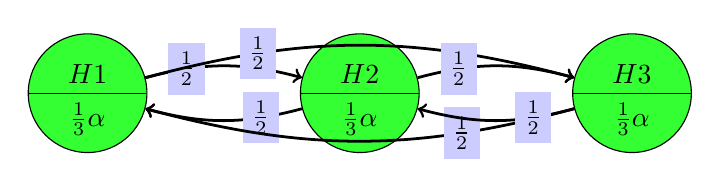
\begin{tikzpicture}[scale=0.7]
\node (H1) at (70bp,-140bp)[draw,circle split,fill=green!80] {$H1$ \nodepart{lower} $\frac{1}{3}\alpha$};
\node (H2) at (210bp,-140bp)[draw,circle split,fill=green!80] {$H2$ \nodepart{lower} $\frac{1}{3}\alpha$};
\node (H3) at (350bp,-140bp)[draw,circle split,fill=green!80] {$H3$ \nodepart{lower} $\frac{1}{3}\alpha$};
\draw [->,line width=1pt] (H1) to[bend left=15] node[near start,fill=blue!20] {$\frac{1}{2}$} (H2);
\draw [->,line width=1pt] (H1) to[bend left=15] node[near start,fill=blue!20] {$\frac{1}{2}$} (H3);
\draw [->,line width=1pt] (H2) to[bend left=15] node[near start,fill=blue!20] {$\frac{1}{2}$} (H1);
\draw [->,line width=1pt] (H2) to[bend left=15] node[near start,fill=blue!20] {$\frac{1}{2}$} (H3);
\draw [->,line width=1pt] (H3) to[bend left=15] node[near start,fill=blue!20] {$\frac{1}{2}$} (H1);
\draw [->,line width=1pt] (H3) to[bend left=15] node[near start,fill=blue!20] {$\frac{1}{2}$} (H2);
\end{tikzpicture}

}  \caption{\label{exampleHolm} Graph representing the
    Bonferroni-Holm-Procedure for three hypotheses.}
\end{figure}

A null hypothesis can be rejected, when the p-value is less than the
alpha level of the corresponding node.  In this case the graph will be
updated and the alpha level of this node is passed according to the
edge weights.

\begin{Example}
  We give an example for the Bonferroni-Holm-Procedure that will
  be used repeatedly throughout this manual. Of course this 
  package is made for more advanced tests (you find a selection in 
  section \ref{caseStudies}),
  but since most readers are already familiar with this procedure,
  for a first introduction of gMCP, we stick to this simple example.  
  
  Let $p_1=0.01$, $p_2=0.07$ and $p_3=0.02$ be three p-values and
  $\alpha=0.05$.  In the first step $H_1$ can be rejected since
  $p_1<\alpha/3$.  The updated graph can be seen in figure
  \ref{exampleHolmP} and now also $H_3$ can be rejected since
  $p_1<\alpha/2$.  Again the graph is updated, but $H_2$
  can not be rejected.
\end{Example}

\begin{figure}[ht]
  \centering
{\tiny
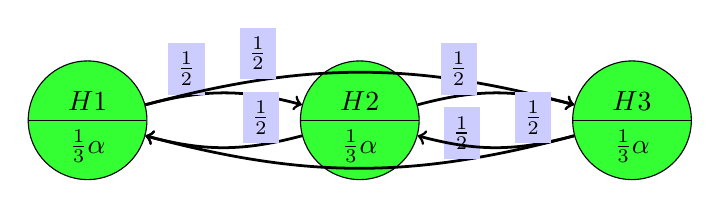
\begin{tikzpicture}[scale=0.7]
\node (H1) at (70bp,-140bp)[draw,circle split,minimum size=1.2cm, fill=green!80] {$H1$ \nodepart{lower} $\frac{1}{3}\alpha$};
\node (H2) at (210bp,-140bp)[draw,circle split,minimum size=1.2cm, fill=green!80] {$H2$ \nodepart{lower} $\frac{1}{3}\alpha$};
\node (H3) at (350bp,-140bp)[draw,circle split,minimum size=1.2cm, fill=green!80] {$H3$ \nodepart{lower} $\frac{1}{3}\alpha$};
\draw [->,line width=1pt] (H1) to[bend left=15] node[near start,above,fill=blue!20] {$\frac{1}{2}$} (H2);
\draw [->,line width=1pt] (H1) to[bend left=15] node[near start,above,fill=blue!20] {$\frac{1}{2}$} (H3);
\draw [->,line width=1pt] (H2) to[bend left=15] node[near start,above,fill=blue!20] {$\frac{1}{2}$} (H1);
\draw [->,line width=1pt] (H2) to[bend left=15] node[near start,above,fill=blue!20] {$\frac{1}{2}$} (H3);
\draw [->,line width=1pt] (H3) to[bend left=15] node[near start,above,fill=blue!20] {$\frac{1}{2}$} (H1);
\draw [->,line width=1pt] (H3) to[bend left=15] node[near start,above,fill=blue!20] {$\frac{1}{2}$} (H2);
\end{tikzpicture}

}$\downarrow$ reject $H_1$\\{\tiny
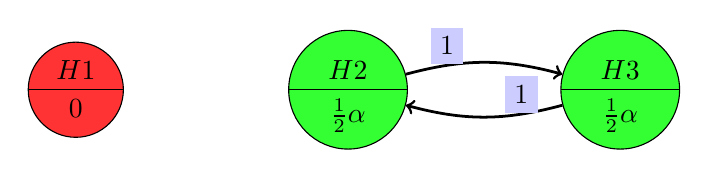
\begin{tikzpicture}[scale=0.7]
\node (H1) at (70bp,-140bp)[draw,circle split,minimum size=1.2cm, fill=red!80] {$H1$ \nodepart{lower} $0$};
\node (H2) at (210bp,-140bp)[draw,circle split,minimum size=1.2cm, fill=green!80] {$H2$ \nodepart{lower} $\frac{1}{2}\alpha$};
\node (H3) at (350bp,-140bp)[draw,circle split,minimum size=1.2cm, fill=green!80] {$H3$ \nodepart{lower} $\frac{1}{2}\alpha$};
\draw [->,line width=1pt] (H2) to[bend left=15] node[near start,above,fill=blue!20] {$1$} (H3);
\draw [->,line width=1pt] (H3) to[bend left=15] node[near start,above,fill=blue!20] {$1$} (H2);
\end{tikzpicture}

}$\downarrow$ reject $H_3$\\{\tiny
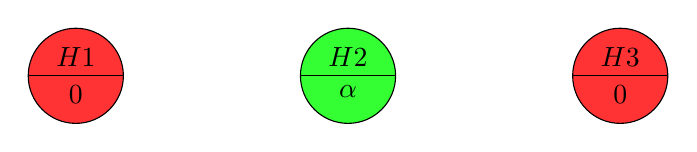
\begin{tikzpicture}[scale=0.7]
\node (H1) at (70bp,-140bp)[draw,circle split,minimum size=1.2cm, fill=red!80] {$H1$ \nodepart{lower} $0$};
\node (H2) at (210bp,-140bp)[draw,circle split,minimum size=1.2cm, fill=green!80] {$H2$ \nodepart{lower} $\alpha$};
\node (H3) at (350bp,-140bp)[draw,circle split,minimum size=1.2cm, fill=red!80] {$H3$ \nodepart{lower} $0$};
\end{tikzpicture}

}  \caption{\label{exampleHolmP} Example showing how two
    null hypotheses can be rejected with p-values $p_1=0.01$,
    $p_2=0.07$ and $p_3=0.02$.}
\end{figure}

Let's reproduce this with the \texttt{gMCP} package. We start R and enter:

\scriptsize
\begin{Hchunk}
\begin{normalsize}
\begin{Hinput}
\ttfamily\noindent
\hlprompt{\usebox{\hlnormalsizeboxgreaterthan}{\ }}\hlfunctioncall{library}\hlkeyword{(}\hlsymbol{gMCP}\hlkeyword{)}\mbox{}
\normalfont
\end{Hinput}


\begin{Hinput}
\ttfamily\noindent
\hlprompt{\usebox{\hlnormalsizeboxgreaterthan}{\ }}\hlfunctioncall{graphGUI}\hlkeyword{(}\hlkeyword{)}\mbox{}
\normalfont
\end{Hinput}


\end{normalsize}
\end{Hchunk}

\normalsize

The GUI seen in Figure \ref{fullGUI} is shown and we select from the
menu "\emph{Example graphs}" the entry "\emph{Bonferroni-Holm Test}".
We enter the three p-values in the respective fields on the right
side.  By clicking on the button with the green arrow we start the
test procedure and can sequentially reject all three hypotheses.

If we don't want to use the GUI we can also use R:

\scriptsize
\begin{Hchunk}
\begin{normalsize}
\begin{Hinput}
\ttfamily\noindent
\hlprompt{\usebox{\hlnormalsizeboxgreaterthan}{\ }}\hlfunctioncall{library}\hlkeyword{(}\hlsymbol{gMCP}\hlkeyword{)}\mbox{}
\normalfont
\end{Hinput}


\begin{Hinput}
\ttfamily\noindent
\hlprompt{\usebox{\hlnormalsizeboxgreaterthan}{\ }}\hlsymbol{graph}{\ }\hlassignement{\usebox{\hlnormalsizeboxlessthan}-}{\ }\hlfunctioncall{createBonferroniHolmGraph}\hlkeyword{(}\hlnumber{3}\hlkeyword{)}\mbox{}
\normalfont
\end{Hinput}


\begin{Hinput}
\ttfamily\noindent
\hlprompt{\usebox{\hlnormalsizeboxgreaterthan}{\ }}\hlfunctioncall{gMCP}\hlkeyword{(}\hlsymbol{graph}\hlkeyword{,}{\ }\hlargument{pvalues}\hlargument{=}\hlfunctioncall{c}\hlkeyword{(}\hlnumber{0.01}\hlkeyword{,}\hlnumber{0.07}\hlkeyword{,}\hlnumber{0.02}\hlkeyword{)}\hlkeyword{,}{\ }\hlargument{alpha}\hlargument{=}\hlnumber{0.05}\hlkeyword{)}\mbox{}
\normalfont
\end{Hinput}

\begin{Houtput}
\ttfamily\noindent
gMCP-Result\hspace*{\fill}\\
\hlstd{}\hspace*{\fill}\\
\hlstd{}Initial{\ }graph:\hspace*{\fill}\\
\hlstd{}A{\ }graphMCP{\ }graph\hspace*{\fill}\\
\hlstd{}H1{\ }(not{\ }rejected,{\ }weight=0.3333)\hspace*{\fill}\\
\hlstd{}H2{\ }(not{\ }rejected,{\ }weight=0.3333)\hspace*{\fill}\\
\hlstd{}H3{\ }(not{\ }rejected,{\ }weight=0.3333)\hspace*{\fill}\\
\hlstd{}Edges:\hspace*{\fill}\\
\hlstd{}H1{\ }{\ }-({\ }1/2{\ })-\usebox{\hlnormalsizeboxgreaterthan}{\ }{\ }H2{\ }\hspace*{\fill}\\
\hlstd{}H1{\ }{\ }-({\ }1/2{\ })-\usebox{\hlnormalsizeboxgreaterthan}{\ }{\ }H3{\ }\hspace*{\fill}\\
\hlstd{}H2{\ }{\ }-({\ }1/2{\ })-\usebox{\hlnormalsizeboxgreaterthan}{\ }{\ }H1{\ }\hspace*{\fill}\\
\hlstd{}H2{\ }{\ }-({\ }1/2{\ })-\usebox{\hlnormalsizeboxgreaterthan}{\ }{\ }H3{\ }\hspace*{\fill}\\
\hlstd{}H3{\ }{\ }-({\ }1/2{\ })-\usebox{\hlnormalsizeboxgreaterthan}{\ }{\ }H1{\ }\hspace*{\fill}\\
\hlstd{}H3{\ }{\ }-({\ }1/2{\ })-\usebox{\hlnormalsizeboxgreaterthan}{\ }{\ }H2{\ }\hspace*{\fill}\\
\hlstd{}\hspace*{\fill}\\
\hlstd{}\hspace*{\fill}\\
\hlstd{}P-values:\hspace*{\fill}\\
\hlstd{}{\ }{\ }H1{\ }{\ }{\ }H2{\ }{\ }{\ }H3{\ }\hspace*{\fill}\\
\hlstd{}0.01{\ }0.07{\ }0.02{\ }\hspace*{\fill}\\
\hlstd{}\hspace*{\fill}\\
\hlstd{}Adjusted{\ }p-values:\hspace*{\fill}\\
\hlstd{}{\ }{\ }H1{\ }{\ }{\ }H2{\ }{\ }{\ }H3{\ }\hspace*{\fill}\\
\hlstd{}0.03{\ }0.07{\ }0.04{\ }\hspace*{\fill}\\
\hlstd{}\hspace*{\fill}\\
\hlstd{}Alpha:{\ }0.05{\ }\hspace*{\fill}\\
\hlstd{}\hspace*{\fill}\\
\hlstd{}Hypothesis{\ }rejected:\hspace*{\fill}\\
\hlstd{}{\ }{\ }{\ }H1{\ }{\ }{\ }{\ }H2{\ }{\ }{\ }{\ }H3{\ }\hspace*{\fill}\\
\hlstd{}{\ }TRUE{\ }FALSE{\ }{\ }TRUE{\ }\hspace*{\fill}\\
\hlstd{}\hspace*{\fill}\\
\hlstd{}Final{\ }graph{\ }after{\ }2{\ }steps:\hspace*{\fill}\\
\hlstd{}A{\ }graphMCP{\ }graph\hspace*{\fill}\\
\hlstd{}H1{\ }(rejected,{\ }weight=0)\hspace*{\fill}\\
\hlstd{}H2{\ }(not{\ }rejected,{\ }weight=1)\hspace*{\fill}\\
\hlstd{}H3{\ }(rejected,{\ }weight=0)\hspace*{\fill}\\
\hlstd{}No{\ }edges.\hspace*{\fill}\hlstd{}\mbox{}
\normalfont
\end{Houtput}

\end{normalsize}
\end{Hchunk}

\normalsize

\section{Creating the graph}

In the first step a graph that describes the multiple test procedures
must be created.

\begin{figure}[ht]
  \centering   
{\tiny
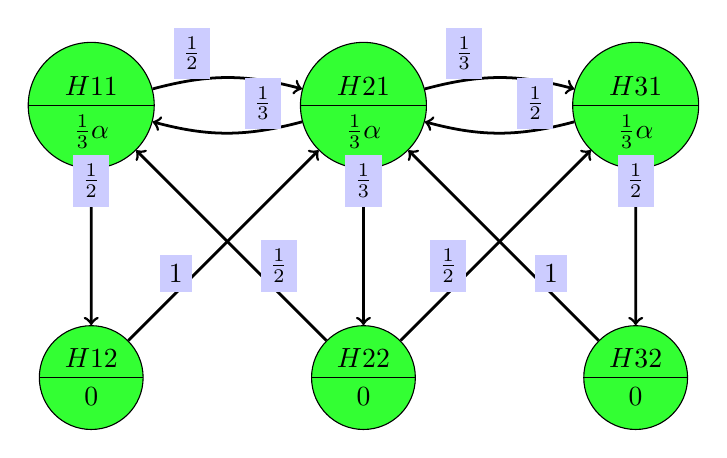
\begin{tikzpicture}[scale=0.7]
\node (H11) at (70bp,-70bp)[draw,circle split,fill=green!80] {$H11$ \nodepart{lower} $\frac{1}{3}\alpha$};
\node (H21) at (210bp,-70bp)[draw,circle split,fill=green!80] {$H21$ \nodepart{lower} $\frac{1}{3}\alpha$};
\node (H31) at (350bp,-70bp)[draw,circle split,fill=green!80] {$H31$ \nodepart{lower} $\frac{1}{3}\alpha$};
\node (H12) at (70bp,-210bp)[draw,circle split,fill=green!80] {$H12$ \nodepart{lower} $0$};
\node (H22) at (210bp,-210bp)[draw,circle split,fill=green!80] {$H22$ \nodepart{lower} $0$};
\node (H32) at (350bp,-210bp)[draw,circle split,fill=green!80] {$H32$ \nodepart{lower} $0$};
\draw [->,line width=1pt] (H11) to[bend left=15] node[near start,above,fill=blue!20] {$\frac{1}{2}$} (H21);
\draw [->,line width=1pt] (H11) to[auto] node[near start,above,fill=blue!20] {$\frac{1}{2}$} (H12);
\draw [->,line width=1pt] (H21) to[bend left=15] node[near start,above,fill=blue!20] {$\frac{1}{3}$} (H11);
\draw [->,line width=1pt] (H21) to[bend left=15] node[near start,above,fill=blue!20] {$\frac{1}{3}$} (H31);
\draw [->,line width=1pt] (H21) to[auto] node[near start,above,fill=blue!20] {$\frac{1}{3}$} (H22);
\draw [->,line width=1pt] (H31) to[bend left=15] node[near start,above,fill=blue!20] {$\frac{1}{2}$} (H21);
\draw [->,line width=1pt] (H31) to[auto] node[near start,above,fill=blue!20] {$\frac{1}{2}$} (H32);
\draw [->,line width=1pt] (H12) to[auto] node[near start,above,fill=blue!20] {$1$} (H21);
\draw [->,line width=1pt] (H22) to[auto] node[near start,above,fill=blue!20] {$\frac{1}{2}$} (H11);
\draw [->,line width=1pt] (H22) to[auto] node[near start,above,fill=blue!20] {$\frac{1}{2}$} (H31);
\draw [->,line width=1pt] (H32) to[auto] node[near start,above,fill=blue!20] {$1$} (H21);
\end{tikzpicture}

}  \caption{\label{exampleGraphBretz} Example graph from \cite{bretzEtAl2009power} that we will create in this vignette.}
\end{figure}

\subsection{Using R}

We build upon the package \texttt{graph} \cite{graph}, more precisely
we declare a new class \texttt{graphMCP} that is a subclass of
\texttt{graphNEL}.  The \texttt{initialize} method of this subclass
differs only in an extra argument \texttt{alpha}, the initial
allocation of the significance level alpha to the individual
hypotheses.  Declaration of the nodes and edges is inherited from
class \texttt{graphNEL}.

As an example we now create the graph from Bretz et
al. \cite{bretzEtAl2009power} that you can see in figure
\ref{exampleGraphBretz}.

\scriptsize
\begin{Hchunk}
\begin{normalsize}
\begin{Hinput}
\ttfamily\noindent
\hlprompt{\usebox{\hlnormalsizeboxgreaterthan}{\ }}\hlsymbol{hnodes}{\ }\hlassignement{\usebox{\hlnormalsizeboxlessthan}-}{\ }\hlfunctioncall{c}\hlkeyword{(}\hlstring{"H11"}\hlkeyword{,}{\ }\hlstring{"H21"}\hlkeyword{,}{\ }\hlstring{"H31"}\hlkeyword{,}{\ }\hlstring{"H12"}\hlkeyword{,}{\ }\hlstring{"H22"}\hlkeyword{,}{\ }\hlstring{"H32"}\hlkeyword{)}\mbox{}
\normalfont
\end{Hinput}


\begin{Hinput}
\ttfamily\noindent
\hlprompt{\usebox{\hlnormalsizeboxgreaterthan}{\ }}\hlsymbol{weights}{\ }\hlassignement{\usebox{\hlnormalsizeboxlessthan}-}{\ }\hlfunctioncall{c}\hlkeyword{(}\hlnumber{1}\hlkeyword{/}\hlnumber{3}\hlkeyword{,}{\ }\hlnumber{1}\hlkeyword{/}\hlnumber{3}\hlkeyword{,}{\ }\hlnumber{1}\hlkeyword{/}\hlnumber{3}\hlkeyword{,}{\ }\hlnumber{0}\hlkeyword{,}{\ }\hlnumber{0}\hlkeyword{,}{\ }\hlnumber{0}\hlkeyword{)}\mbox{}
\normalfont
\end{Hinput}


\begin{Hinput}
\ttfamily\noindent
\hlprompt{\usebox{\hlnormalsizeboxgreaterthan}{\ }}\hlsymbol{edges}{\ }\hlassignement{\usebox{\hlnormalsizeboxlessthan}-}{\ }\hlfunctioncall{list}\hlkeyword{(}\hlkeyword{)}\mbox{}
\normalfont
\end{Hinput}


\begin{Hinput}
\ttfamily\noindent
\hlprompt{\usebox{\hlnormalsizeboxgreaterthan}{\ }}\hlsymbol{edges}\hlkeyword{[[}\hlstring{"H11"}\hlkeyword{]}\hlkeyword{]}{\ }\hlassignement{\usebox{\hlnormalsizeboxlessthan}-}{\ }\hlfunctioncall{list}\hlkeyword{(}\hlargument{edges}\hlargument{=}\hlfunctioncall{c}\hlkeyword{(}\hlstring{"H21"}\hlkeyword{,}\hlstring{"H12"}\hlkeyword{)}\hlkeyword{,}{\ }\hlargument{weights}\hlargument{=}\hlfunctioncall{c}\hlkeyword{(}\hlnumber{1}\hlkeyword{/}\hlnumber{2}\hlkeyword{,}{\ }\hlnumber{1}\hlkeyword{/}\hlnumber{2}\hlkeyword{)}\hlkeyword{)}\mbox{}
\normalfont
\end{Hinput}


\begin{Hinput}
\ttfamily\noindent
\hlprompt{\usebox{\hlnormalsizeboxgreaterthan}{\ }}\hlsymbol{edges}\hlkeyword{[[}\hlstring{"H21"}\hlkeyword{]}\hlkeyword{]}{\ }\hlassignement{\usebox{\hlnormalsizeboxlessthan}-}{\ }\hlfunctioncall{list}\hlkeyword{(}\hlargument{edges}\hlargument{=}\hlfunctioncall{c}\hlkeyword{(}\hlstring{"H11"}\hlkeyword{,}\hlstring{"H31"}\hlkeyword{,}\hlstring{"H22"}\hlkeyword{)}\hlkeyword{,}{\ }\hlargument{weights}\hlargument{=}\hlfunctioncall{c}\hlkeyword{(}\hlnumber{1}\hlkeyword{/}\hlnumber{3}\hlkeyword{,}{\ }\hlnumber{1}\hlkeyword{/}\hlnumber{3}\hlkeyword{,}{\ }\hlnumber{1}\hlkeyword{/}\hlnumber{3}\hlkeyword{)}\hlkeyword{)}\mbox{}
\normalfont
\end{Hinput}


\begin{Hinput}
\ttfamily\noindent
\hlprompt{\usebox{\hlnormalsizeboxgreaterthan}{\ }}\hlsymbol{edges}\hlkeyword{[[}\hlstring{"H31"}\hlkeyword{]}\hlkeyword{]}{\ }\hlassignement{\usebox{\hlnormalsizeboxlessthan}-}{\ }\hlfunctioncall{list}\hlkeyword{(}\hlargument{edges}\hlargument{=}\hlfunctioncall{c}\hlkeyword{(}\hlstring{"H21"}\hlkeyword{,}\hlstring{"H32"}\hlkeyword{)}\hlkeyword{,}{\ }\hlargument{weights}\hlargument{=}\hlfunctioncall{c}\hlkeyword{(}\hlnumber{1}\hlkeyword{/}\hlnumber{2}\hlkeyword{,}{\ }\hlnumber{1}\hlkeyword{/}\hlnumber{2}\hlkeyword{)}\hlkeyword{)}\mbox{}
\normalfont
\end{Hinput}


\begin{Hinput}
\ttfamily\noindent
\hlprompt{\usebox{\hlnormalsizeboxgreaterthan}{\ }}\hlsymbol{edges}\hlkeyword{[[}\hlstring{"H12"}\hlkeyword{]}\hlkeyword{]}{\ }\hlassignement{\usebox{\hlnormalsizeboxlessthan}-}{\ }\hlfunctioncall{list}\hlkeyword{(}\hlargument{edges}\hlargument{=}\hlstring{"H21"}\hlkeyword{,}{\ }\hlargument{weights}\hlargument{=}\hlnumber{1}\hlkeyword{)}\mbox{}
\normalfont
\end{Hinput}


\begin{Hinput}
\ttfamily\noindent
\hlprompt{\usebox{\hlnormalsizeboxgreaterthan}{\ }}\hlsymbol{edges}\hlkeyword{[[}\hlstring{"H22"}\hlkeyword{]}\hlkeyword{]}{\ }\hlassignement{\usebox{\hlnormalsizeboxlessthan}-}{\ }\hlfunctioncall{list}\hlkeyword{(}\hlargument{edges}\hlargument{=}\hlfunctioncall{c}\hlkeyword{(}\hlstring{"H11"}\hlkeyword{,}\hlstring{"H31"}\hlkeyword{)}\hlkeyword{,}{\ }\hlargument{weights}\hlargument{=}\hlfunctioncall{c}\hlkeyword{(}\hlnumber{1}\hlkeyword{/}\hlnumber{2}\hlkeyword{,}{\ }\hlnumber{1}\hlkeyword{/}\hlnumber{2}\hlkeyword{)}\hlkeyword{)}\mbox{}
\normalfont
\end{Hinput}


\begin{Hinput}
\ttfamily\noindent
\hlprompt{\usebox{\hlnormalsizeboxgreaterthan}{\ }}\hlsymbol{edges}\hlkeyword{[[}\hlstring{"H32"}\hlkeyword{]}\hlkeyword{]}{\ }\hlassignement{\usebox{\hlnormalsizeboxlessthan}-}{\ }\hlfunctioncall{list}\hlkeyword{(}\hlargument{edges}\hlargument{=}\hlstring{"H21"}\hlkeyword{,}{\ }\hlargument{weights}\hlargument{=}\hlnumber{1}\hlkeyword{)}\mbox{}
\normalfont
\end{Hinput}


\begin{Hinput}
\ttfamily\noindent
\hlprompt{\usebox{\hlnormalsizeboxgreaterthan}{\ }}\hlsymbol{graph}{\ }\hlassignement{\usebox{\hlnormalsizeboxlessthan}-}{\ }\hlfunctioncall{new}\hlkeyword{(}\hlstring{"graphMCP"}\hlkeyword{,}{\ }\hlargument{nodes}\hlargument{=}\hlsymbol{hnodes}\hlkeyword{,}{\ }\hlargument{edgeL}\hlargument{=}\hlsymbol{edges}\hlkeyword{,}{\ }\hlargument{weights}\hlargument{=}\hlsymbol{weights}\hlkeyword{)}\mbox{}
\normalfont
\end{Hinput}


\end{normalsize}
\end{Hchunk}

\normalsize

Let's print the newly created graph:

\scriptsize
\begin{Hchunk}
\begin{normalsize}
\begin{Hinput}
\ttfamily\noindent
\hlprompt{\usebox{\hlnormalsizeboxgreaterthan}{\ }}\hlfunctioncall{print}\hlkeyword{(}\hlsymbol{graph}\hlkeyword{)}\mbox{}
\normalfont
\end{Hinput}

\begin{Houtput}
\ttfamily\noindent
A{\ }graphMCP{\ }graph\hspace*{\fill}\\
\hlstd{}H11{\ }(not{\ }rejected,{\ }weight=0.3333)\hspace*{\fill}\\
\hlstd{}H21{\ }(not{\ }rejected,{\ }weight=0.3333)\hspace*{\fill}\\
\hlstd{}H31{\ }(not{\ }rejected,{\ }weight=0.3333)\hspace*{\fill}\\
\hlstd{}H12{\ }(not{\ }rejected,{\ }weight=0)\hspace*{\fill}\\
\hlstd{}H22{\ }(not{\ }rejected,{\ }weight=0)\hspace*{\fill}\\
\hlstd{}H32{\ }(not{\ }rejected,{\ }weight=0)\hspace*{\fill}\\
\hlstd{}Edges:\hspace*{\fill}\\
\hlstd{}H11{\ }{\ }-({\ }1/2{\ })-\usebox{\hlnormalsizeboxgreaterthan}{\ }{\ }H21{\ }\hspace*{\fill}\\
\hlstd{}H11{\ }{\ }-({\ }1/2{\ })-\usebox{\hlnormalsizeboxgreaterthan}{\ }{\ }H12{\ }\hspace*{\fill}\\
\hlstd{}H21{\ }{\ }-({\ }1/3{\ })-\usebox{\hlnormalsizeboxgreaterthan}{\ }{\ }H11{\ }\hspace*{\fill}\\
\hlstd{}H21{\ }{\ }-({\ }1/3{\ })-\usebox{\hlnormalsizeboxgreaterthan}{\ }{\ }H31{\ }\hspace*{\fill}\\
\hlstd{}H21{\ }{\ }-({\ }1/3{\ })-\usebox{\hlnormalsizeboxgreaterthan}{\ }{\ }H22{\ }\hspace*{\fill}\\
\hlstd{}H31{\ }{\ }-({\ }1/2{\ })-\usebox{\hlnormalsizeboxgreaterthan}{\ }{\ }H21{\ }\hspace*{\fill}\\
\hlstd{}H31{\ }{\ }-({\ }1/2{\ })-\usebox{\hlnormalsizeboxgreaterthan}{\ }{\ }H32{\ }\hspace*{\fill}\\
\hlstd{}H12{\ }{\ }-({\ }1{\ })-\usebox{\hlnormalsizeboxgreaterthan}{\ }{\ }H21{\ }\hspace*{\fill}\\
\hlstd{}H22{\ }{\ }-({\ }1/2{\ })-\usebox{\hlnormalsizeboxgreaterthan}{\ }{\ }H11{\ }\hspace*{\fill}\\
\hlstd{}H22{\ }{\ }-({\ }1/2{\ })-\usebox{\hlnormalsizeboxgreaterthan}{\ }{\ }H31{\ }\hspace*{\fill}\\
\hlstd{}H32{\ }{\ }-({\ }1{\ })-\usebox{\hlnormalsizeboxgreaterthan}{\ }{\ }H21{\ }\hspace*{\fill}\hlstd{}\mbox{}
\normalfont
\end{Houtput}

\end{normalsize}
\end{Hchunk}

\normalsize

Since we also want to visualize the graph, we use the method
\texttt{nodeRenderInfo}\index{nodeRenderInfo} from package \texttt{graph} to set appropriate
x- and y-coordinates in the renderInfo.  (We are compatible to the
renderInfo usage from package Rgraphviz \cite{Rgraphviz}.)

\scriptsize
\begin{Hchunk}
\begin{normalsize}
\begin{Hinput}
\ttfamily\noindent
\hlprompt{\usebox{\hlnormalsizeboxgreaterthan}{\ }}\hlsymbol{nodeX}{\ }\hlassignement{\usebox{\hlnormalsizeboxlessthan}-}{\ }\hlfunctioncall{c}\hlkeyword{(}\hlargument{H11}\hlargument{=}\hlnumber{100}\hlkeyword{,}{\ }\hlargument{H21}\hlargument{=}\hlnumber{300}\hlkeyword{,}{\ }\hlargument{H31}\hlargument{=}\hlnumber{500}\hlkeyword{,}{\ }\hlargument{H12}\hlargument{=}\hlnumber{100}\hlkeyword{,}{\ }\hlargument{H22}\hlargument{=}\hlnumber{300}\hlkeyword{,}{\ }\hlargument{H32}\hlargument{=}\hlnumber{500}\hlkeyword{)}\mbox{}
\normalfont
\end{Hinput}


\begin{Hinput}
\ttfamily\noindent
\hlprompt{\usebox{\hlnormalsizeboxgreaterthan}{\ }}\hlsymbol{nodeY}{\ }\hlassignement{\usebox{\hlnormalsizeboxlessthan}-}{\ }\hlfunctioncall{c}\hlkeyword{(}\hlargument{H11}\hlargument{=}\hlnumber{100}\hlkeyword{,}{\ }\hlargument{H21}\hlargument{=}\hlnumber{100}\hlkeyword{,}{\ }\hlargument{H31}\hlargument{=}\hlnumber{100}\hlkeyword{,}{\ }\hlargument{H12}\hlargument{=}\hlnumber{300}\hlkeyword{,}{\ }\hlargument{H22}\hlargument{=}\hlnumber{300}\hlkeyword{,}{\ }\hlargument{H32}\hlargument{=}\hlnumber{300}\hlkeyword{)}\mbox{}
\normalfont
\end{Hinput}


\begin{Hinput}
\ttfamily\noindent
\hlprompt{\usebox{\hlnormalsizeboxgreaterthan}{\ }}\hlfunctioncall{nodeRenderInfo}\hlkeyword{(}\hlsymbol{graph}\hlkeyword{)}{\ }\hlassignement{\usebox{\hlnormalsizeboxlessthan}-}{\ }\hlfunctioncall{list}\hlkeyword{(}\hlargument{nodeX}\hlargument{=}\hlsymbol{nodeX}\hlkeyword{,}{\ }\hlargument{nodeY}\hlargument{=}\hlsymbol{nodeY}\hlkeyword{)}\mbox{}
\normalfont
\end{Hinput}


\end{normalsize}
\end{Hchunk}

\normalsize

For placement of the nodes in a matrix pattern, the function \texttt{placeNodes} is helpful.
The following code does the same as the three lines of R code above.  

\scriptsize
\begin{Hchunk}
\begin{normalsize}
\begin{Hinput}
\ttfamily\noindent
\hlprompt{\usebox{\hlnormalsizeboxgreaterthan}{\ }}\hlsymbol{graph}{\ }\hlassignement{\usebox{\hlnormalsizeboxlessthan}-}{\ }\hlfunctioncall{placeNodes}\hlkeyword{(}\hlsymbol{graph}\hlkeyword{,}{\ }\hlargument{nrow}\hlargument{=}\hlnumber{2}\hlkeyword{)}\mbox{}
\normalfont
\end{Hinput}


\end{normalsize}
\end{Hchunk}

\normalsize

Coordinates are interpretated as pixels in the GUI and big points in
{\LaTeX} (72 bp = 1 inch).\index{coordinates}

Let's take a look at the graph in {\LaTeX} rendered with TikZ
\cite{TikZ}\index{TikZ} (you can see the compiled result in figure
\ref{exampleGraphBretz}):

\scriptsize
%\lstset{language=[LaTeX]TeX}
%\begin{lstlisting}
\begin{Hchunk}
\begin{normalsize}
\begin{Hinput}
\ttfamily\noindent
\hlprompt{\usebox{\hlnormalsizeboxgreaterthan}{\ }}\hlfunctioncall{cat}\hlkeyword{(}\hlfunctioncall{graph2latex}\hlkeyword{(}\hlsymbol{graph}\hlkeyword{)}\hlkeyword{)}\mbox{}
\normalfont
\end{Hinput}

\begin{Houtput}
\ttfamily\noindent
\usebox{\hlnormalsizeboxbackslash}begin\usebox{\hlnormalsizeboxopenbrace}tikzpicture\usebox{\hlnormalsizeboxclosebrace}[scale=1]\hspace*{\fill}\\
\hlstd{}\usebox{\hlnormalsizeboxbackslash}node{\ }(H11){\ }at{\ }(100bp,-100bp)[draw,circle{\ }split,fill=green!80]{\ }\usebox{\hlnormalsizeboxopenbrace}\usebox{\hlnormalsizeboxdollar}H11\usebox{\hlnormalsizeboxdollar}{\ }\usebox{\hlnormalsizeboxbackslash}nodepart\usebox{\hlnormalsizeboxopenbrace}lower\usebox{\hlnormalsizeboxclosebrace}{\ }\usebox{\hlnormalsizeboxdollar}\usebox{\hlnormalsizeboxbackslash}frac\usebox{\hlnormalsizeboxopenbrace}1\usebox{\hlnormalsizeboxclosebrace}\usebox{\hlnormalsizeboxopenbrace}3\usebox{\hlnormalsizeboxclosebrace}\usebox{\hlnormalsizeboxbackslash}alpha\usebox{\hlnormalsizeboxdollar}\usebox{\hlnormalsizeboxclosebrace};\hspace*{\fill}\\
\hlstd{}\usebox{\hlnormalsizeboxbackslash}node{\ }(H21){\ }at{\ }(300bp,-100bp)[draw,circle{\ }split,fill=green!80]{\ }\usebox{\hlnormalsizeboxopenbrace}\usebox{\hlnormalsizeboxdollar}H21\usebox{\hlnormalsizeboxdollar}{\ }\usebox{\hlnormalsizeboxbackslash}nodepart\usebox{\hlnormalsizeboxopenbrace}lower\usebox{\hlnormalsizeboxclosebrace}{\ }\usebox{\hlnormalsizeboxdollar}\usebox{\hlnormalsizeboxbackslash}frac\usebox{\hlnormalsizeboxopenbrace}1\usebox{\hlnormalsizeboxclosebrace}\usebox{\hlnormalsizeboxopenbrace}3\usebox{\hlnormalsizeboxclosebrace}\usebox{\hlnormalsizeboxbackslash}alpha\usebox{\hlnormalsizeboxdollar}\usebox{\hlnormalsizeboxclosebrace};\hspace*{\fill}\\
\hlstd{}\usebox{\hlnormalsizeboxbackslash}node{\ }(H31){\ }at{\ }(500bp,-100bp)[draw,circle{\ }split,fill=green!80]{\ }\usebox{\hlnormalsizeboxopenbrace}\usebox{\hlnormalsizeboxdollar}H31\usebox{\hlnormalsizeboxdollar}{\ }\usebox{\hlnormalsizeboxbackslash}nodepart\usebox{\hlnormalsizeboxopenbrace}lower\usebox{\hlnormalsizeboxclosebrace}{\ }\usebox{\hlnormalsizeboxdollar}\usebox{\hlnormalsizeboxbackslash}frac\usebox{\hlnormalsizeboxopenbrace}1\usebox{\hlnormalsizeboxclosebrace}\usebox{\hlnormalsizeboxopenbrace}3\usebox{\hlnormalsizeboxclosebrace}\usebox{\hlnormalsizeboxbackslash}alpha\usebox{\hlnormalsizeboxdollar}\usebox{\hlnormalsizeboxclosebrace};\hspace*{\fill}\\
\hlstd{}\usebox{\hlnormalsizeboxbackslash}node{\ }(H12){\ }at{\ }(100bp,-300bp)[draw,circle{\ }split,fill=green!80]{\ }\usebox{\hlnormalsizeboxopenbrace}\usebox{\hlnormalsizeboxdollar}H12\usebox{\hlnormalsizeboxdollar}{\ }\usebox{\hlnormalsizeboxbackslash}nodepart\usebox{\hlnormalsizeboxopenbrace}lower\usebox{\hlnormalsizeboxclosebrace}{\ }\usebox{\hlnormalsizeboxdollar}0\usebox{\hlnormalsizeboxdollar}\usebox{\hlnormalsizeboxclosebrace};\hspace*{\fill}\\
\hlstd{}\usebox{\hlnormalsizeboxbackslash}node{\ }(H22){\ }at{\ }(300bp,-300bp)[draw,circle{\ }split,fill=green!80]{\ }\usebox{\hlnormalsizeboxopenbrace}\usebox{\hlnormalsizeboxdollar}H22\usebox{\hlnormalsizeboxdollar}{\ }\usebox{\hlnormalsizeboxbackslash}nodepart\usebox{\hlnormalsizeboxopenbrace}lower\usebox{\hlnormalsizeboxclosebrace}{\ }\usebox{\hlnormalsizeboxdollar}0\usebox{\hlnormalsizeboxdollar}\usebox{\hlnormalsizeboxclosebrace};\hspace*{\fill}\\
\hlstd{}\usebox{\hlnormalsizeboxbackslash}node{\ }(H32){\ }at{\ }(500bp,-300bp)[draw,circle{\ }split,fill=green!80]{\ }\usebox{\hlnormalsizeboxopenbrace}\usebox{\hlnormalsizeboxdollar}H32\usebox{\hlnormalsizeboxdollar}{\ }\usebox{\hlnormalsizeboxbackslash}nodepart\usebox{\hlnormalsizeboxopenbrace}lower\usebox{\hlnormalsizeboxclosebrace}{\ }\usebox{\hlnormalsizeboxdollar}0\usebox{\hlnormalsizeboxdollar}\usebox{\hlnormalsizeboxclosebrace};\hspace*{\fill}\\
\hlstd{}\usebox{\hlnormalsizeboxbackslash}draw{\ }[-\usebox{\hlnormalsizeboxgreaterthan},line{\ }width=1pt]{\ }(H11){\ }to[bend{\ }left=15]{\ }node[near{\ }start,above,fill=blue!20]{\ }\usebox{\hlnormalsizeboxopenbrace}\usebox{\hlnormalsizeboxdollar}\usebox{\hlnormalsizeboxbackslash}frac\usebox{\hlnormalsizeboxopenbrace}1\usebox{\hlnormalsizeboxclosebrace}\usebox{\hlnormalsizeboxopenbrace}2\usebox{\hlnormalsizeboxclosebrace}\usebox{\hlnormalsizeboxdollar}\usebox{\hlnormalsizeboxclosebrace}{\ }(H21);\hspace*{\fill}\\
\hlstd{}\usebox{\hlnormalsizeboxbackslash}draw{\ }[-\usebox{\hlnormalsizeboxgreaterthan},line{\ }width=1pt]{\ }(H11){\ }to[auto]{\ }node[near{\ }start,above,fill=blue!20]{\ }\usebox{\hlnormalsizeboxopenbrace}\usebox{\hlnormalsizeboxdollar}\usebox{\hlnormalsizeboxbackslash}frac\usebox{\hlnormalsizeboxopenbrace}1\usebox{\hlnormalsizeboxclosebrace}\usebox{\hlnormalsizeboxopenbrace}2\usebox{\hlnormalsizeboxclosebrace}\usebox{\hlnormalsizeboxdollar}\usebox{\hlnormalsizeboxclosebrace}{\ }(H12);\hspace*{\fill}\\
\hlstd{}\usebox{\hlnormalsizeboxbackslash}draw{\ }[-\usebox{\hlnormalsizeboxgreaterthan},line{\ }width=1pt]{\ }(H21){\ }to[bend{\ }left=15]{\ }node[near{\ }start,above,fill=blue!20]{\ }\usebox{\hlnormalsizeboxopenbrace}\usebox{\hlnormalsizeboxdollar}\usebox{\hlnormalsizeboxbackslash}frac\usebox{\hlnormalsizeboxopenbrace}1\usebox{\hlnormalsizeboxclosebrace}\usebox{\hlnormalsizeboxopenbrace}3\usebox{\hlnormalsizeboxclosebrace}\usebox{\hlnormalsizeboxdollar}\usebox{\hlnormalsizeboxclosebrace}{\ }(H11);\hspace*{\fill}\\
\hlstd{}\usebox{\hlnormalsizeboxbackslash}draw{\ }[-\usebox{\hlnormalsizeboxgreaterthan},line{\ }width=1pt]{\ }(H21){\ }to[bend{\ }left=15]{\ }node[near{\ }start,above,fill=blue!20]{\ }\usebox{\hlnormalsizeboxopenbrace}\usebox{\hlnormalsizeboxdollar}\usebox{\hlnormalsizeboxbackslash}frac\usebox{\hlnormalsizeboxopenbrace}1\usebox{\hlnormalsizeboxclosebrace}\usebox{\hlnormalsizeboxopenbrace}3\usebox{\hlnormalsizeboxclosebrace}\usebox{\hlnormalsizeboxdollar}\usebox{\hlnormalsizeboxclosebrace}{\ }(H31);\hspace*{\fill}\\
\hlstd{}\usebox{\hlnormalsizeboxbackslash}draw{\ }[-\usebox{\hlnormalsizeboxgreaterthan},line{\ }width=1pt]{\ }(H21){\ }to[auto]{\ }node[near{\ }start,above,fill=blue!20]{\ }\usebox{\hlnormalsizeboxopenbrace}\usebox{\hlnormalsizeboxdollar}\usebox{\hlnormalsizeboxbackslash}frac\usebox{\hlnormalsizeboxopenbrace}1\usebox{\hlnormalsizeboxclosebrace}\usebox{\hlnormalsizeboxopenbrace}3\usebox{\hlnormalsizeboxclosebrace}\usebox{\hlnormalsizeboxdollar}\usebox{\hlnormalsizeboxclosebrace}{\ }(H22);\hspace*{\fill}\\
\hlstd{}\usebox{\hlnormalsizeboxbackslash}draw{\ }[-\usebox{\hlnormalsizeboxgreaterthan},line{\ }width=1pt]{\ }(H31){\ }to[bend{\ }left=15]{\ }node[near{\ }start,above,fill=blue!20]{\ }\usebox{\hlnormalsizeboxopenbrace}\usebox{\hlnormalsizeboxdollar}\usebox{\hlnormalsizeboxbackslash}frac\usebox{\hlnormalsizeboxopenbrace}1\usebox{\hlnormalsizeboxclosebrace}\usebox{\hlnormalsizeboxopenbrace}2\usebox{\hlnormalsizeboxclosebrace}\usebox{\hlnormalsizeboxdollar}\usebox{\hlnormalsizeboxclosebrace}{\ }(H21);\hspace*{\fill}\\
\hlstd{}\usebox{\hlnormalsizeboxbackslash}draw{\ }[-\usebox{\hlnormalsizeboxgreaterthan},line{\ }width=1pt]{\ }(H31){\ }to[auto]{\ }node[near{\ }start,above,fill=blue!20]{\ }\usebox{\hlnormalsizeboxopenbrace}\usebox{\hlnormalsizeboxdollar}\usebox{\hlnormalsizeboxbackslash}frac\usebox{\hlnormalsizeboxopenbrace}1\usebox{\hlnormalsizeboxclosebrace}\usebox{\hlnormalsizeboxopenbrace}2\usebox{\hlnormalsizeboxclosebrace}\usebox{\hlnormalsizeboxdollar}\usebox{\hlnormalsizeboxclosebrace}{\ }(H32);\hspace*{\fill}\\
\hlstd{}\usebox{\hlnormalsizeboxbackslash}draw{\ }[-\usebox{\hlnormalsizeboxgreaterthan},line{\ }width=1pt]{\ }(H12){\ }to[auto]{\ }node[near{\ }start,above,fill=blue!20]{\ }\usebox{\hlnormalsizeboxopenbrace}\usebox{\hlnormalsizeboxdollar}1\usebox{\hlnormalsizeboxdollar}\usebox{\hlnormalsizeboxclosebrace}{\ }(H21);\hspace*{\fill}\\
\hlstd{}\usebox{\hlnormalsizeboxbackslash}draw{\ }[-\usebox{\hlnormalsizeboxgreaterthan},line{\ }width=1pt]{\ }(H22){\ }to[auto]{\ }node[near{\ }start,above,fill=blue!20]{\ }\usebox{\hlnormalsizeboxopenbrace}\usebox{\hlnormalsizeboxdollar}\usebox{\hlnormalsizeboxbackslash}frac\usebox{\hlnormalsizeboxopenbrace}1\usebox{\hlnormalsizeboxclosebrace}\usebox{\hlnormalsizeboxopenbrace}2\usebox{\hlnormalsizeboxclosebrace}\usebox{\hlnormalsizeboxdollar}\usebox{\hlnormalsizeboxclosebrace}{\ }(H11);\hspace*{\fill}\\
\hlstd{}\usebox{\hlnormalsizeboxbackslash}draw{\ }[-\usebox{\hlnormalsizeboxgreaterthan},line{\ }width=1pt]{\ }(H22){\ }to[auto]{\ }node[near{\ }start,above,fill=blue!20]{\ }\usebox{\hlnormalsizeboxopenbrace}\usebox{\hlnormalsizeboxdollar}\usebox{\hlnormalsizeboxbackslash}frac\usebox{\hlnormalsizeboxopenbrace}1\usebox{\hlnormalsizeboxclosebrace}\usebox{\hlnormalsizeboxopenbrace}2\usebox{\hlnormalsizeboxclosebrace}\usebox{\hlnormalsizeboxdollar}\usebox{\hlnormalsizeboxclosebrace}{\ }(H31);\hspace*{\fill}\\
\hlstd{}\usebox{\hlnormalsizeboxbackslash}draw{\ }[-\usebox{\hlnormalsizeboxgreaterthan},line{\ }width=1pt]{\ }(H32){\ }to[auto]{\ }node[near{\ }start,above,fill=blue!20]{\ }\usebox{\hlnormalsizeboxopenbrace}\usebox{\hlnormalsizeboxdollar}1\usebox{\hlnormalsizeboxdollar}\usebox{\hlnormalsizeboxclosebrace}{\ }(H21);\hspace*{\fill}\\
\hlstd{}\usebox{\hlnormalsizeboxbackslash}end\usebox{\hlnormalsizeboxopenbrace}tikzpicture\usebox{\hlnormalsizeboxclosebrace}\hspace*{\fill}\hlstd{}\mbox{}
\normalfont
\end{Houtput}

\end{normalsize}
\end{Hchunk}

%\end{lstlisting}
\normalsize

We can even change the position of the edge labels for further fine
tuning of the graphical representation.  With the following command we
place the label for the edge from \texttt{H1} to \texttt{H2} at
position (200, 80):

\scriptsize
\begin{Hchunk}
\begin{normalsize}
\begin{Hinput}
\ttfamily\noindent
\hlprompt{\usebox{\hlnormalsizeboxgreaterthan}{\ }}\hlfunctioncall{edgeData}\hlkeyword{(}\hlsymbol{graph}\hlkeyword{,}{\ }\hlstring{"H11"}\hlkeyword{,}{\ }\hlstring{"H21"}\hlkeyword{,}{\ }\hlstring{"labelX"}\hlkeyword{)}{\ }\hlassignement{\usebox{\hlnormalsizeboxlessthan}-}{\ }\hlnumber{200}\mbox{}
\normalfont
\end{Hinput}


\begin{Hinput}
\ttfamily\noindent
\hlprompt{\usebox{\hlnormalsizeboxgreaterthan}{\ }}\hlfunctioncall{edgeData}\hlkeyword{(}\hlsymbol{graph}\hlkeyword{,}{\ }\hlstring{"H11"}\hlkeyword{,}{\ }\hlstring{"H21"}\hlkeyword{,}{\ }\hlstring{"labelY"}\hlkeyword{)}{\ }\hlassignement{\usebox{\hlnormalsizeboxlessthan}-}{\ }\hlnumber{80}\mbox{}
\normalfont
\end{Hinput}


\end{normalsize}
\end{Hchunk}

\normalsize

\subsubsection{graph2matrix and matrix2graph}\index{graph2matrix}\index{matrix2graph}

We can also constuct a graph from a given adjacency matrix via the
command \texttt{matrix2graph}:

\scriptsize
\begin{Hchunk}
\begin{normalsize}
\begin{Hinput}
\ttfamily\noindent
\hlprompt{\usebox{\hlnormalsizeboxgreaterthan}{\ }}\hlcomment{\usebox{\hlnormalsizeboxhash}{\ }Bonferroni-Holm:}\hspace*{\fill}\\
\hlstd{}\hlprompt{\usebox{\hlnormalsizeboxgreaterthan}{\ }}\hlsymbol{m}{\ }\hlassignement{\usebox{\hlnormalsizeboxlessthan}-}{\ }\hlfunctioncall{matrix}\hlkeyword{(}\hlfunctioncall{rep}\hlkeyword{(}\hlnumber{1}\hlkeyword{/}\hlnumber{3}\hlkeyword{,}{\ }\hlnumber{16}\hlkeyword{)}\hlkeyword{,}{\ }\hlargument{nrow}\hlargument{=}\hlnumber{4}\hlkeyword{)}\mbox{}
\normalfont
\end{Hinput}


\begin{Hinput}
\ttfamily\noindent
\hlprompt{\usebox{\hlnormalsizeboxgreaterthan}{\ }}\hlfunctioncall{diag}\hlkeyword{(}\hlsymbol{m}\hlkeyword{)}{\ }\hlassignement{\usebox{\hlnormalsizeboxlessthan}-}{\ }\hlfunctioncall{c}\hlkeyword{(}\hlnumber{0}\hlkeyword{,}{\ }\hlnumber{0}\hlkeyword{,}{\ }\hlnumber{0}\hlkeyword{,}{\ }\hlnumber{0}\hlkeyword{)}\mbox{}
\normalfont
\end{Hinput}


\begin{Hinput}
\ttfamily\noindent
\hlprompt{\usebox{\hlnormalsizeboxgreaterthan}{\ }}\hlsymbol{graph}{\ }\hlassignement{\usebox{\hlnormalsizeboxlessthan}-}{\ }\hlfunctioncall{matrix2graph}\hlkeyword{(}\hlsymbol{m}\hlkeyword{)}\mbox{}
\normalfont
\end{Hinput}


\begin{Hinput}
\ttfamily\noindent
\hlprompt{\usebox{\hlnormalsizeboxgreaterthan}{\ }}\hlfunctioncall{print}\hlkeyword{(}\hlsymbol{graph}\hlkeyword{)}\mbox{}
\normalfont
\end{Hinput}

\begin{Houtput}
\ttfamily\noindent
A{\ }graphMCP{\ }graph\hspace*{\fill}\\
\hlstd{}H1{\ }(not{\ }rejected,{\ }weight=0.25)\hspace*{\fill}\\
\hlstd{}H2{\ }(not{\ }rejected,{\ }weight=0.25)\hspace*{\fill}\\
\hlstd{}H3{\ }(not{\ }rejected,{\ }weight=0.25)\hspace*{\fill}\\
\hlstd{}H4{\ }(not{\ }rejected,{\ }weight=0.25)\hspace*{\fill}\\
\hlstd{}Edges:\hspace*{\fill}\\
\hlstd{}H1{\ }{\ }-({\ }1/3{\ })-\usebox{\hlnormalsizeboxgreaterthan}{\ }{\ }H2{\ }\hspace*{\fill}\\
\hlstd{}H1{\ }{\ }-({\ }1/3{\ })-\usebox{\hlnormalsizeboxgreaterthan}{\ }{\ }H3{\ }\hspace*{\fill}\\
\hlstd{}H1{\ }{\ }-({\ }1/3{\ })-\usebox{\hlnormalsizeboxgreaterthan}{\ }{\ }H4{\ }\hspace*{\fill}\\
\hlstd{}H2{\ }{\ }-({\ }1/3{\ })-\usebox{\hlnormalsizeboxgreaterthan}{\ }{\ }H1{\ }\hspace*{\fill}\\
\hlstd{}H2{\ }{\ }-({\ }1/3{\ })-\usebox{\hlnormalsizeboxgreaterthan}{\ }{\ }H3{\ }\hspace*{\fill}\\
\hlstd{}H2{\ }{\ }-({\ }1/3{\ })-\usebox{\hlnormalsizeboxgreaterthan}{\ }{\ }H4{\ }\hspace*{\fill}\\
\hlstd{}H3{\ }{\ }-({\ }1/3{\ })-\usebox{\hlnormalsizeboxgreaterthan}{\ }{\ }H1{\ }\hspace*{\fill}\\
\hlstd{}H3{\ }{\ }-({\ }1/3{\ })-\usebox{\hlnormalsizeboxgreaterthan}{\ }{\ }H2{\ }\hspace*{\fill}\\
\hlstd{}H3{\ }{\ }-({\ }1/3{\ })-\usebox{\hlnormalsizeboxgreaterthan}{\ }{\ }H4{\ }\hspace*{\fill}\\
\hlstd{}H4{\ }{\ }-({\ }1/3{\ })-\usebox{\hlnormalsizeboxgreaterthan}{\ }{\ }H1{\ }\hspace*{\fill}\\
\hlstd{}H4{\ }{\ }-({\ }1/3{\ })-\usebox{\hlnormalsizeboxgreaterthan}{\ }{\ }H2{\ }\hspace*{\fill}\\
\hlstd{}H4{\ }{\ }-({\ }1/3{\ })-\usebox{\hlnormalsizeboxgreaterthan}{\ }{\ }H3{\ }\hspace*{\fill}\hlstd{}\mbox{}
\normalfont
\end{Houtput}

\begin{Hinput}
\ttfamily\noindent
\hlprompt{\usebox{\hlnormalsizeboxgreaterthan}{\ }}\hlfunctioncall{graph2matrix}\hlkeyword{(}\hlsymbol{graph}\hlkeyword{)}\mbox{}
\normalfont
\end{Hinput}

\begin{Houtput}
\ttfamily\noindent
{\ }{\ }{\ }{\ }{\ }{\ }{\ }H1{\ }{\ }{\ }{\ }{\ }H2{\ }{\ }{\ }{\ }{\ }H3{\ }{\ }{\ }{\ }{\ }H4\hspace*{\fill}\\
\hlstd{}H1{\ }0.0000{\ }0.3333{\ }0.3333{\ }0.3333\hspace*{\fill}\\
\hlstd{}H2{\ }0.3333{\ }0.0000{\ }0.3333{\ }0.3333\hspace*{\fill}\\
\hlstd{}H3{\ }0.3333{\ }0.3333{\ }0.0000{\ }0.3333\hspace*{\fill}\\
\hlstd{}H4{\ }0.3333{\ }0.3333{\ }0.3333{\ }0.0000\hspace*{\fill}\hlstd{}\mbox{}
\normalfont
\end{Houtput}

\end{normalsize}
\end{Hchunk}

\normalsize

\subsection{Using the GUI}

The creation of \texttt{graphMCP} objects as seen in the last section 
with basic R commands is very straight forward,
but still takes some time and typos may occur.  More convenient for
the average user is the use of the graphical user interface for
creating and editing MCP graphs that the \texttt{gMCP} package
includes.

It is called by the command \texttt{graphGUI()} and takes as optional
argument a variable name, given as a character string, of the graph to
edit or under which a newly created \texttt{graphMCP} object will be
available from the R command line.

\scriptsize
\begin{Hchunk}
\begin{normalsize}
\begin{Hinput}
\ttfamily\noindent
\hlprompt{\usebox{\hlnormalsizeboxgreaterthan}{\ }}\hlfunctioncall{graphGUI}\hlkeyword{(}\hlstring{"graph"}\hlkeyword{)}\mbox{}
\normalfont
\end{Hinput}


\end{normalsize}
\end{Hchunk}

\normalsize

\begin{figure}[ht]
  \centering    
  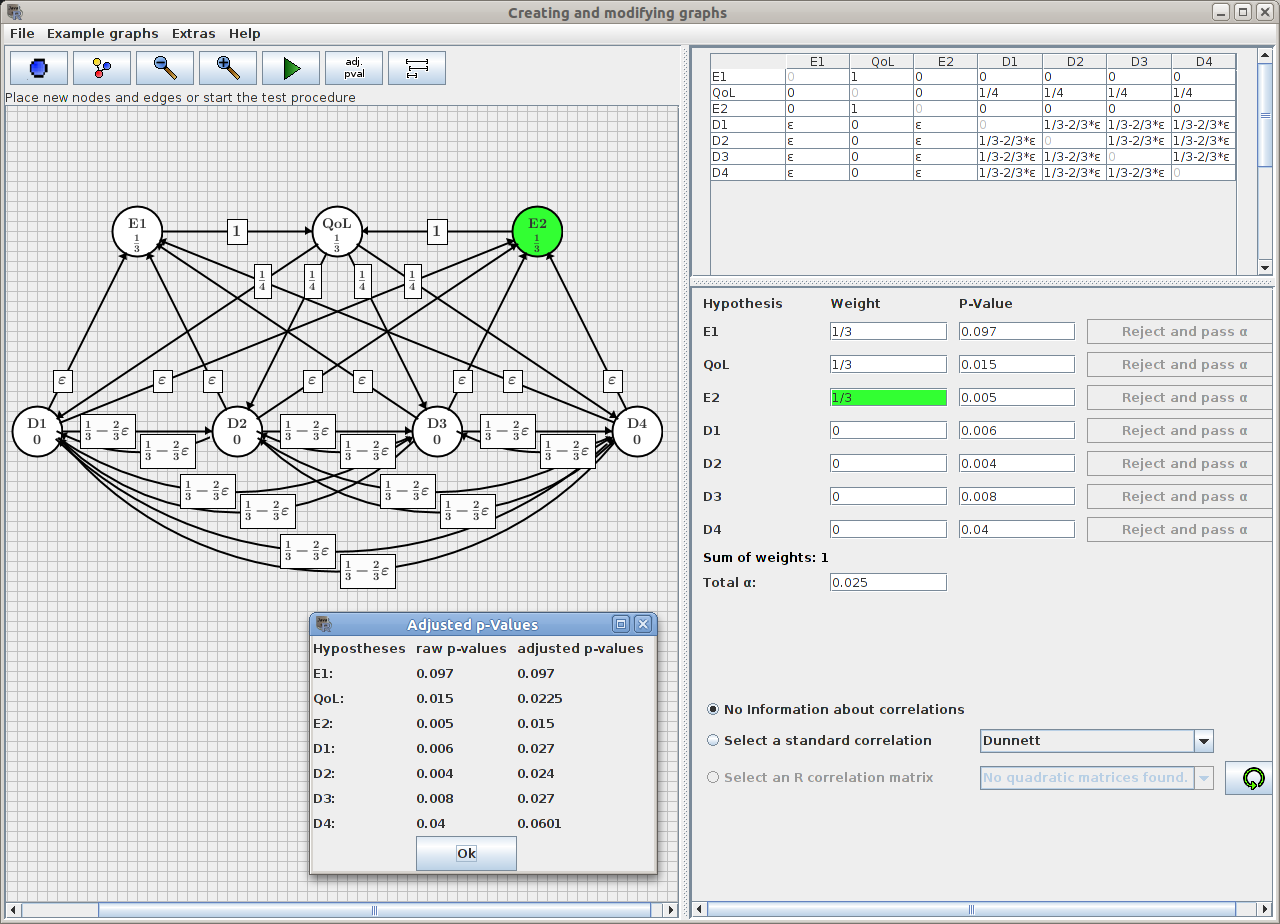
\includegraphics[width=0.95\textwidth]{pictures/FullFeaturedGUI.png}      
  \caption{\label{fullGUI} The graphical user interface allows testing, calculation of confidence intervals and adjusted p-values.}
\end{figure}

Let's take a look at the icon panel:


\includegraphics[width=0.5cm]{pictures/vertex.png} This button lets
you add a new node to the graph.  After pressing the button click
somewhere on the graph panel and a new node will appear at this place.


\includegraphics[width=0.5cm]{pictures/edge.png} This button lets you
add a new edge between two nodes.  After pressing the button click on
the node the edge should start and after that on the node the edge
should end.


\includegraphics[width=0.5cm]{pictures/zoom_in.png}

\includegraphics[width=0.5cm]{pictures/zoom_out.png} For really big
graphs the ability to zoom in and out is usefull.


\includegraphics[width=0.5cm]{pictures/StartTesting.png}

\includegraphics[width=0.5cm]{pictures/Reset.png} Starts the testing
procedure / goes back to the graph modification.


\includegraphics[width=0.5cm]{pictures/adjPval.png} Calculates the
adjusted p-values.


\includegraphics[width=0.5cm]{pictures/confint2.png} Calculates
simultaneous confidence intervals.

With drag and drop you can move nodes and also adjust edges.

\section{The sequentially rejective MTP}

For a full description of the sequentially rejective multiple testing
procedure take a look at Bretz et al. \cite{bretzEtAl2009graphical}. 

\subsection{Using R}

You can either specify each rejection step yourself or simply use the 
method \texttt{gMCP}:

\scriptsize
\begin{Hchunk}
\begin{normalsize}
\begin{Hinput}
\ttfamily\noindent
\hlprompt{\usebox{\hlnormalsizeboxgreaterthan}{\ }}\hlsymbol{graph}{\ }\hlassignement{\usebox{\hlnormalsizeboxlessthan}-}{\ }\hlfunctioncall{createGraphFromBretzEtAl}\hlkeyword{(}\hlkeyword{)}\mbox{}
\normalfont
\end{Hinput}


\begin{Hinput}
\ttfamily\noindent
\hlprompt{\usebox{\hlnormalsizeboxgreaterthan}{\ }}\hlcomment{\usebox{\hlnormalsizeboxhash}{\ }We{\ }can{\ }reject{\ }a{\ }single{\ }node:}\hspace*{\fill}\\
\hlstd{}\hlprompt{\usebox{\hlnormalsizeboxgreaterthan}{\ }}\hlfunctioncall{print}\hlkeyword{(}\hlfunctioncall{rejectNode}\hlkeyword{(}\hlsymbol{graph}\hlkeyword{,}{\ }\hlstring{"H11"}\hlkeyword{)}\hlkeyword{)}\mbox{}
\normalfont
\end{Hinput}

\begin{Houtput}
\ttfamily\noindent
A{\ }graphMCP{\ }graph\hspace*{\fill}\\
\hlstd{}H11{\ }(rejected,{\ }weight=0)\hspace*{\fill}\\
\hlstd{}H21{\ }(not{\ }rejected,{\ }weight=0.5)\hspace*{\fill}\\
\hlstd{}H31{\ }(not{\ }rejected,{\ }weight=0.3333)\hspace*{\fill}\\
\hlstd{}H12{\ }(not{\ }rejected,{\ }weight=0.1667)\hspace*{\fill}\\
\hlstd{}H22{\ }(not{\ }rejected,{\ }weight=0)\hspace*{\fill}\\
\hlstd{}H32{\ }(not{\ }rejected,{\ }weight=0)\hspace*{\fill}\\
\hlstd{}Edges:\hspace*{\fill}\\
\hlstd{}H21{\ }{\ }-({\ }2/5{\ })-\usebox{\hlnormalsizeboxgreaterthan}{\ }{\ }H31{\ }\hspace*{\fill}\\
\hlstd{}H21{\ }{\ }-({\ }2/5{\ })-\usebox{\hlnormalsizeboxgreaterthan}{\ }{\ }H22{\ }\hspace*{\fill}\\
\hlstd{}H21{\ }{\ }-({\ }1/5{\ })-\usebox{\hlnormalsizeboxgreaterthan}{\ }{\ }H12{\ }\hspace*{\fill}\\
\hlstd{}H31{\ }{\ }-({\ }1/2{\ })-\usebox{\hlnormalsizeboxgreaterthan}{\ }{\ }H21{\ }\hspace*{\fill}\\
\hlstd{}H31{\ }{\ }-({\ }1/2{\ })-\usebox{\hlnormalsizeboxgreaterthan}{\ }{\ }H32{\ }\hspace*{\fill}\\
\hlstd{}H12{\ }{\ }-({\ }1{\ })-\usebox{\hlnormalsizeboxgreaterthan}{\ }{\ }H21{\ }\hspace*{\fill}\\
\hlstd{}H22{\ }{\ }-({\ }1/2{\ })-\usebox{\hlnormalsizeboxgreaterthan}{\ }{\ }H31{\ }\hspace*{\fill}\\
\hlstd{}H22{\ }{\ }-({\ }1/4{\ })-\usebox{\hlnormalsizeboxgreaterthan}{\ }{\ }H21{\ }\hspace*{\fill}\\
\hlstd{}H22{\ }{\ }-({\ }1/4{\ })-\usebox{\hlnormalsizeboxgreaterthan}{\ }{\ }H12{\ }\hspace*{\fill}\\
\hlstd{}H32{\ }{\ }-({\ }1{\ })-\usebox{\hlnormalsizeboxgreaterthan}{\ }{\ }H21{\ }\hspace*{\fill}\hlstd{}\mbox{}
\normalfont
\end{Houtput}

\begin{Hinput}
\ttfamily\noindent
\hlprompt{\usebox{\hlnormalsizeboxgreaterthan}{\ }}\hlcomment{\usebox{\hlnormalsizeboxhash}{\ }Or{\ }given{\ }a{\ }vector{\ }of{\ }pvalues{\ }let{\ }the{\ }function{\ }gMCP{\ }do{\ }all{\ }the{\ }work:{\ }{\ }}\hspace*{\fill}\\
\hlstd{}\hlprompt{\usebox{\hlnormalsizeboxgreaterthan}{\ }}\hlsymbol{pvalues}{\ }\hlassignement{\usebox{\hlnormalsizeboxlessthan}-}{\ }\hlfunctioncall{c}\hlkeyword{(}\hlnumber{0.1}\hlkeyword{,}{\ }\hlnumber{0.008}\hlkeyword{,}{\ }\hlnumber{0.005}\hlkeyword{,}{\ }\hlnumber{0.15}\hlkeyword{,}{\ }\hlnumber{0.04}\hlkeyword{,}{\ }\hlnumber{0.006}\hlkeyword{)}\mbox{}
\normalfont
\end{Hinput}


\begin{Hinput}
\ttfamily\noindent
\hlprompt{\usebox{\hlnormalsizeboxgreaterthan}{\ }}\hlsymbol{result}{\ }\hlassignement{\usebox{\hlnormalsizeboxlessthan}-}{\ }\hlfunctioncall{gMCP}\hlkeyword{(}\hlsymbol{graph}\hlkeyword{,}{\ }\hlsymbol{pvalues}\hlkeyword{)}\mbox{}
\normalfont
\end{Hinput}


\begin{Hinput}
\ttfamily\noindent
\hlprompt{\usebox{\hlnormalsizeboxgreaterthan}{\ }}\hlfunctioncall{print}\hlkeyword{(}\hlsymbol{result}\hlkeyword{)}\mbox{}
\normalfont
\end{Hinput}

\begin{Houtput}
\ttfamily\noindent
gMCP-Result\hspace*{\fill}\\
\hlstd{}\hspace*{\fill}\\
\hlstd{}Initial{\ }graph:\hspace*{\fill}\\
\hlstd{}A{\ }graphMCP{\ }graph\hspace*{\fill}\\
\hlstd{}H11{\ }(not{\ }rejected,{\ }weight=0.3333)\hspace*{\fill}\\
\hlstd{}H21{\ }(not{\ }rejected,{\ }weight=0.3333)\hspace*{\fill}\\
\hlstd{}H31{\ }(not{\ }rejected,{\ }weight=0.3333)\hspace*{\fill}\\
\hlstd{}H12{\ }(not{\ }rejected,{\ }weight=0)\hspace*{\fill}\\
\hlstd{}H22{\ }(not{\ }rejected,{\ }weight=0)\hspace*{\fill}\\
\hlstd{}H32{\ }(not{\ }rejected,{\ }weight=0)\hspace*{\fill}\\
\hlstd{}Edges:\hspace*{\fill}\\
\hlstd{}H11{\ }{\ }-({\ }1/2{\ })-\usebox{\hlnormalsizeboxgreaterthan}{\ }{\ }H21{\ }\hspace*{\fill}\\
\hlstd{}H11{\ }{\ }-({\ }1/2{\ })-\usebox{\hlnormalsizeboxgreaterthan}{\ }{\ }H12{\ }\hspace*{\fill}\\
\hlstd{}H21{\ }{\ }-({\ }1/3{\ })-\usebox{\hlnormalsizeboxgreaterthan}{\ }{\ }H11{\ }\hspace*{\fill}\\
\hlstd{}H21{\ }{\ }-({\ }1/3{\ })-\usebox{\hlnormalsizeboxgreaterthan}{\ }{\ }H31{\ }\hspace*{\fill}\\
\hlstd{}H21{\ }{\ }-({\ }1/3{\ })-\usebox{\hlnormalsizeboxgreaterthan}{\ }{\ }H22{\ }\hspace*{\fill}\\
\hlstd{}H31{\ }{\ }-({\ }1/2{\ })-\usebox{\hlnormalsizeboxgreaterthan}{\ }{\ }H21{\ }\hspace*{\fill}\\
\hlstd{}H31{\ }{\ }-({\ }1/2{\ })-\usebox{\hlnormalsizeboxgreaterthan}{\ }{\ }H32{\ }\hspace*{\fill}\\
\hlstd{}H12{\ }{\ }-({\ }1{\ })-\usebox{\hlnormalsizeboxgreaterthan}{\ }{\ }H21{\ }\hspace*{\fill}\\
\hlstd{}H22{\ }{\ }-({\ }1/2{\ })-\usebox{\hlnormalsizeboxgreaterthan}{\ }{\ }H11{\ }\hspace*{\fill}\\
\hlstd{}H22{\ }{\ }-({\ }1/2{\ })-\usebox{\hlnormalsizeboxgreaterthan}{\ }{\ }H31{\ }\hspace*{\fill}\\
\hlstd{}H32{\ }{\ }-({\ }1{\ })-\usebox{\hlnormalsizeboxgreaterthan}{\ }{\ }H21{\ }\hspace*{\fill}\\
\hlstd{}\hspace*{\fill}\\
\hlstd{}\hspace*{\fill}\\
\hlstd{}P-values:\hspace*{\fill}\\
\hlstd{}{\ }{\ }H11{\ }{\ }{\ }H21{\ }{\ }{\ }H31{\ }{\ }{\ }H12{\ }{\ }{\ }H22{\ }{\ }{\ }H32{\ }\hspace*{\fill}\\
\hlstd{}0.100{\ }0.008{\ }0.005{\ }0.150{\ }0.040{\ }0.006{\ }\hspace*{\fill}\\
\hlstd{}\hspace*{\fill}\\
\hlstd{}Adjusted{\ }p-values:\hspace*{\fill}\\
\hlstd{}{\ }{\ }{\ }H11{\ }{\ }{\ }{\ }H21{\ }{\ }{\ }{\ }H31{\ }{\ }{\ }{\ }H12{\ }{\ }{\ }{\ }H22{\ }{\ }{\ }{\ }H32{\ }\hspace*{\fill}\\
\hlstd{}0.1200{\ }0.0160{\ }0.0150{\ }0.1500{\ }0.1200{\ }0.0225{\ }\hspace*{\fill}\\
\hlstd{}\hspace*{\fill}\\
\hlstd{}Alpha:{\ }0.05{\ }\hspace*{\fill}\\
\hlstd{}\hspace*{\fill}\\
\hlstd{}Hypothesis{\ }rejected:\hspace*{\fill}\\
\hlstd{}{\ }{\ }H11{\ }{\ }{\ }H21{\ }{\ }{\ }H31{\ }{\ }{\ }H12{\ }{\ }{\ }H22{\ }{\ }{\ }H32{\ }\hspace*{\fill}\\
\hlstd{}FALSE{\ }{\ }TRUE{\ }{\ }TRUE{\ }FALSE{\ }FALSE{\ }{\ }TRUE{\ }\hspace*{\fill}\\
\hlstd{}\hspace*{\fill}\\
\hlstd{}Final{\ }graph{\ }after{\ }3{\ }steps:\hspace*{\fill}\\
\hlstd{}A{\ }graphMCP{\ }graph\hspace*{\fill}\\
\hlstd{}H11{\ }(not{\ }rejected,{\ }weight=0.6667)\hspace*{\fill}\\
\hlstd{}H21{\ }(rejected,{\ }weight=0)\hspace*{\fill}\\
\hlstd{}H31{\ }(rejected,{\ }weight=0)\hspace*{\fill}\\
\hlstd{}H12{\ }(not{\ }rejected,{\ }weight=0)\hspace*{\fill}\\
\hlstd{}H22{\ }(not{\ }rejected,{\ }weight=0.3333)\hspace*{\fill}\\
\hlstd{}H32{\ }(rejected,{\ }weight=0)\hspace*{\fill}\\
\hlstd{}Edges:\hspace*{\fill}\\
\hlstd{}H11{\ }{\ }-({\ }2/3{\ })-\usebox{\hlnormalsizeboxgreaterthan}{\ }{\ }H12{\ }\hspace*{\fill}\\
\hlstd{}H11{\ }{\ }-({\ }1/3{\ })-\usebox{\hlnormalsizeboxgreaterthan}{\ }{\ }H22{\ }\hspace*{\fill}\\
\hlstd{}H12{\ }{\ }-({\ }1/2{\ })-\usebox{\hlnormalsizeboxgreaterthan}{\ }{\ }H11{\ }\hspace*{\fill}\\
\hlstd{}H12{\ }{\ }-({\ }1/2{\ })-\usebox{\hlnormalsizeboxgreaterthan}{\ }{\ }H22{\ }\hspace*{\fill}\\
\hlstd{}H22{\ }{\ }-({\ }1{\ })-\usebox{\hlnormalsizeboxgreaterthan}{\ }{\ }H11{\ }\hspace*{\fill}\hlstd{}\mbox{}
\normalfont
\end{Houtput}

\end{normalsize}
\end{Hchunk}

\normalsize

We can create a TikZ graphic from the last graph with 
\texttt{graph2latex(result@graphs[[4]])} that is shown in figure \ref{finalstate}.

\begin{figure}[ht]
  \centering   
{\tiny
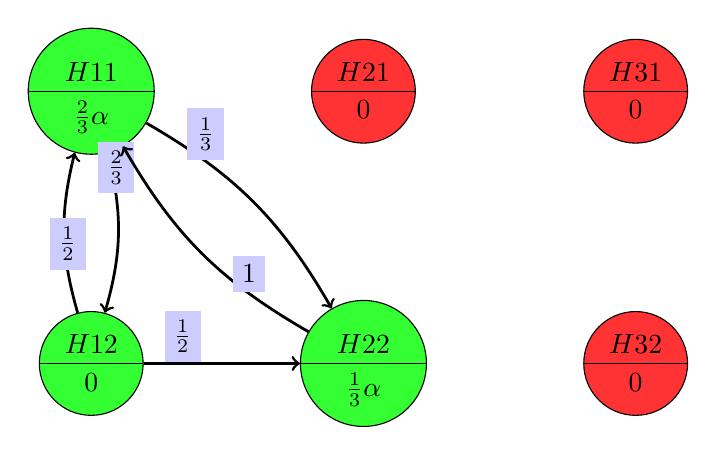
\begin{tikzpicture}[scale=0.7]
\node (H11) at (70bp,-70bp)[draw,circle split,fill=green!80] {$H11$ \nodepart{lower} $\frac{2}{3}\alpha$};
\node (H21) at (210bp,-70bp)[draw,circle split,fill=red!80] {$H21$ \nodepart{lower} $0$};
\node (H31) at (350bp,-70bp)[draw,circle split,fill=red!80] {$H31$ \nodepart{lower} $0$};
\node (H12) at (70bp,-210bp)[draw,circle split,fill=green!80] {$H12$ \nodepart{lower} $0$};
\node (H22) at (210bp,-210bp)[draw,circle split,fill=green!80] {$H22$ \nodepart{lower} $\frac{1}{3}\alpha$};
\node (H32) at (350bp,-210bp)[draw,circle split,fill=red!80] {$H32$ \nodepart{lower} $0$};
\draw [->,line width=1pt] (H11) to[bend left=15] node[near start,above,fill=blue!20] {$\frac{2}{3}$} (H12);
\draw [->,line width=1pt] (H11) to[bend left=15] node[near start,above,fill=blue!20] {$\frac{1}{3}$} (H22);
\draw [->,line width=1pt] (H12) to[bend left=15] node[near start,above,fill=blue!20] {$\frac{1}{2}$} (H11);
\draw [->,line width=1pt] (H12) to[auto] node[near start,above,fill=blue!20] {$\frac{1}{2}$} (H22);
\draw [->,line width=1pt] (H22) to[bend left=15] node[near start,above,fill=blue!20] {$1$} (H11);
\end{tikzpicture}

}  \caption{\label{finalstate}Final graph from the test procedure after rejection of $H_{21}$, $H_{31}$ and $H_{32}$.}
\end{figure}

The command \texttt{gMCPReport}\index{report generation} generates a full report of the testing
procedure:

\scriptsize
\begin{Hchunk}
\begin{normalsize}
\begin{Hinput}
\ttfamily\noindent
\hlprompt{\usebox{\hlnormalsizeboxgreaterthan}{\ }}\hlfunctioncall{gMCPReport}\hlkeyword{(}\hlsymbol{result}\hlkeyword{,}{\ }\hlstring{"Report.tex"}\hlkeyword{)}\mbox{}
\normalfont
\end{Hinput}


\end{normalsize}
\end{Hchunk}

\normalsize

\subsubsection{Adjusted p-values and simultaneous confidence intervals}\index{adjusted p-values}\index{simultaneous confidence intervals}

Also adjusted p-values and simultaneous confidence intervals can be computed.


Let's assume the tests for hypotheses $H1:\;\theta_1\leq0$,
$H2:\;\theta_2\leq0$ and $H3:\;\theta_3\leq0$ are three t-tests with degree
of freedom 9.  The estimates are
$\hat\theta_1=0.981$,
$\hat\theta_2=1.089$ and
$\hat\theta_3=0.8706$, the sample standard deviations
$s_1=0.876$,
$s_2=1.291$ and
$s_3=0.8571$ the t-statistics
$3.541$, $2.666$ and
$3.212$ and the corresponding p-values $0.0063$, 
$0.02577$ and
$0.01062$.  We want to adjust for multiple testing
by using the Bonferroni-Holm-Procedure with $\alpha=0.025$.

\scriptsize
\begin{Hchunk}
\begin{normalsize}
\begin{Hinput}
\ttfamily\noindent
\hlprompt{\usebox{\hlnormalsizeboxgreaterthan}{\ }}\hlcomment{\usebox{\hlnormalsizeboxhash}{\ }Estimates:}\hspace*{\fill}\\
\hlstd{}\hlprompt{\usebox{\hlnormalsizeboxgreaterthan}{\ }}\hlsymbol{est}{\ }\hlassignement{\usebox{\hlnormalsizeboxlessthan}-}{\ }\hlfunctioncall{c}\hlkeyword{(}\hlstring{"H1"}\hlargument{=}\hlnumber{0.860382}\hlkeyword{,}{\ }\hlstring{"H2"}\hlargument{=}\hlnumber{0.9161474}\hlkeyword{,}{\ }\hlstring{"H3"}\hlargument{=}\hlnumber{0.9732953}\hlkeyword{)}\mbox{}
\normalfont
\end{Hinput}


\begin{Hinput}
\ttfamily\noindent
\hlprompt{\usebox{\hlnormalsizeboxgreaterthan}{\ }}\hlcomment{\usebox{\hlnormalsizeboxhash}{\ }Sample{\ }standard{\ }deviations:}\hspace*{\fill}\\
\hlstd{}\hlprompt{\usebox{\hlnormalsizeboxgreaterthan}{\ }}\hlsymbol{ssd}{\ }\hlassignement{\usebox{\hlnormalsizeboxlessthan}-}{\ }\hlfunctioncall{c}\hlkeyword{(}\hlstring{"H1"}\hlargument{=}\hlnumber{0.8759528}\hlkeyword{,}{\ }\hlstring{"H2"}\hlargument{=}\hlnumber{1.291310}\hlkeyword{,}{\ }\hlstring{"H3"}\hlargument{=}\hlnumber{0.8570892}\hlkeyword{)}\mbox{}
\normalfont
\end{Hinput}


\begin{Hinput}
\ttfamily\noindent
\hlprompt{\usebox{\hlnormalsizeboxgreaterthan}{\ }}\hlsymbol{pval}{\ }\hlassignement{\usebox{\hlnormalsizeboxlessthan}-}{\ }\hlfunctioncall{c}\hlkeyword{(}\hlnumber{0.01260}\hlkeyword{,}{\ }\hlnumber{0.05154}\hlkeyword{,}{\ }\hlnumber{0.02124}\hlkeyword{)}\hlkeyword{/}\hlnumber{2}\mbox{}
\normalfont
\end{Hinput}


\begin{Hinput}
\ttfamily\noindent
\hlprompt{\usebox{\hlnormalsizeboxgreaterthan}{\ }}\hlfunctioncall{simConfint}\hlkeyword{(}\hlfunctioncall{createBonferroniHolmGraph}\hlkeyword{(}\hlnumber{3}\hlkeyword{)}\hlkeyword{,}{\ }\hlargument{pvalues}\hlargument{=}\hlsymbol{pval}\hlkeyword{,}\hspace*{\fill}\\
\hlstd{}\hlprompt{+{\ }}{\ }{\ }{\ }{\ }{\ }{\ }{\ }{\ }{\ }{\ }{\ }{\ }{\ }{\ }{\ }{\ }\hlargument{confint}\hlargument{=}\hlkeyword{function}\hlkeyword{(}\hlformalargs{node}\hlkeyword{,}{\ }\hlformalargs{alpha}\hlkeyword{)}{\ }\hlkeyword{\usebox{\hlnormalsizeboxopenbrace}}\hspace*{\fill}\\
\hlstd{}\hlprompt{+{\ }}{\ }{\ }{\ }{\ }{\ }{\ }{\ }{\ }{\ }{\ }{\ }{\ }{\ }{\ }{\ }{\ }{\ }{\ }{\ }{\ }{\ }{\ }{\ }{\ }\hlfunctioncall{c}\hlkeyword{(}\hlsymbol{est}\hlkeyword{[}\hlsymbol{node}\hlkeyword{]}\hlkeyword{-}\hlfunctioncall{qt}\hlkeyword{(}\hlnumber{1}\hlkeyword{-}\hlsymbol{alpha}\hlkeyword{,}\hlargument{df}\hlargument{=}\hlnumber{9}\hlkeyword{)}\hlkeyword{*}\hlsymbol{ssd}\hlkeyword{[}\hlsymbol{node}\hlkeyword{]}\hlkeyword{/}\hlfunctioncall{sqrt}\hlkeyword{(}\hlnumber{10}\hlkeyword{)}\hlkeyword{,}{\ }\hlnumber{Inf}\hlkeyword{)}\hspace*{\fill}\\
\hlstd{}\hlprompt{+{\ }}{\ }{\ }{\ }{\ }{\ }{\ }{\ }{\ }{\ }{\ }{\ }{\ }{\ }{\ }{\ }{\ }\hlkeyword{\usebox{\hlnormalsizeboxclosebrace}}\hlkeyword{,}{\ }\hlargument{alpha}\hlargument{=}\hlnumber{0.025}\hlkeyword{,}{\ }\hlargument{mu}\hlargument{=}\hlnumber{0}\hlkeyword{,}{\ }\hlargument{alternative}\hlargument{=}\hlstring{"greater"}\hlkeyword{)}\mbox{}
\normalfont
\end{Hinput}

\begin{Houtput}
\ttfamily\noindent
{\ }{\ }{\ }lower{\ }bound{\ }upper{\ }bound\hspace*{\fill}\\
\hlstd{}H1{\ }{\ }{\ }{\ }{\ }{\ }0.0000{\ }{\ }{\ }{\ }{\ }{\ }{\ }{\ }{\ }Inf\hspace*{\fill}\\
\hlstd{}H2{\ }{\ }{\ }{\ }{\ }-0.0076{\ }{\ }{\ }{\ }{\ }{\ }{\ }{\ }{\ }Inf\hspace*{\fill}\\
\hlstd{}H3{\ }{\ }{\ }{\ }{\ }{\ }0.0000{\ }{\ }{\ }{\ }{\ }{\ }{\ }{\ }{\ }Inf\hspace*{\fill}\hlstd{}\mbox{}
\normalfont
\end{Houtput}

\begin{Hinput}
\ttfamily\noindent
\hlprompt{\usebox{\hlnormalsizeboxgreaterthan}{\ }}\hlcomment{\usebox{\hlnormalsizeboxhash}{\ }Note{\ }that{\ }the{\ }sample{\ }standard{\ }deviations{\ }will{\ }be{\ }calculated{\ }from{\ }the{\ }pvalues{\ }and{\ }estimates.}\hspace*{\fill}\\
\hlstd{}\hlprompt{\usebox{\hlnormalsizeboxgreaterthan}{\ }}\hlcomment{\usebox{\hlnormalsizeboxhash}{\ }For{\ }example{\ }by{\ }estimates/dist(pvalues){\ }for{\ }alternative="less".}\hspace*{\fill}\\
\hlstd{}\hlprompt{\usebox{\hlnormalsizeboxgreaterthan}{\ }}\hlfunctioncall{simConfint}\hlkeyword{(}\hlfunctioncall{createBonferroniHolmGraph}\hlkeyword{(}\hlnumber{3}\hlkeyword{)}\hlkeyword{,}{\ }\hlargument{pvalues}\hlargument{=}\hlsymbol{pval}\hlkeyword{,}\hspace*{\fill}\\
\hlstd{}\hlprompt{+{\ }}{\ }{\ }{\ }{\ }{\ }{\ }{\ }{\ }{\ }{\ }{\ }{\ }{\ }{\ }{\ }{\ }\hlargument{confint}\hlargument{=}\hlstring{"t"}\hlkeyword{,}{\ }\hlargument{df}\hlargument{=}\hlnumber{9}\hlkeyword{,}{\ }\hlargument{estimates}\hlargument{=}\hlsymbol{est}\hlkeyword{,}{\ }\hlargument{alpha}\hlargument{=}\hlnumber{0.025}\hlkeyword{,}{\ }\hlargument{alternative}\hlargument{=}\hlstring{"greater"}\hlkeyword{)}\mbox{}
\normalfont
\end{Hinput}

\begin{Houtput}
\ttfamily\noindent
{\ }{\ }{\ }{\ }{\ }lower{\ }bound{\ }upper{\ }bound\hspace*{\fill}\\
\hlstd{}[1,]{\ }{\ }{\ }{\ }0.000000{\ }{\ }{\ }{\ }{\ }{\ }{\ }{\ }{\ }Inf\hspace*{\fill}\\
\hlstd{}[2,]{\ }{\ }{\ }-0.007581{\ }{\ }{\ }{\ }{\ }{\ }{\ }{\ }{\ }Inf\hspace*{\fill}\\
\hlstd{}[3,]{\ }{\ }{\ }{\ }0.000000{\ }{\ }{\ }{\ }{\ }{\ }{\ }{\ }{\ }Inf\hspace*{\fill}\hlstd{}\mbox{}
\normalfont
\end{Houtput}

\end{normalsize}
\end{Hchunk}

\normalsize

\subsection{Using the GUI}

\begin{figure}[ht]
  \centering    
  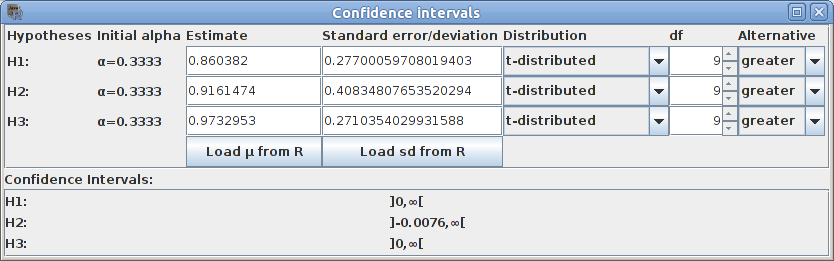
\includegraphics[width=0.7\textwidth]{pictures/CIDialog.png}      
  \caption{\label{CIDialog} For normal and t-distributions simultaneous CI can be calculated by the GUI.}
\end{figure}


Use the following two buttons:

\includegraphics[width=1cm]{pictures/adjPval_b.png}

\includegraphics[width=1cm]{pictures/confint2_b.png}

See \cite{Bretz11}.

\section{Weighted parametric tests}

\begin{figure}[ht]
  \centering    
  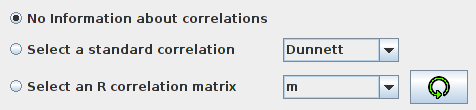
\includegraphics[width=0.7\textwidth]{pictures/correlated.png}      
  \caption{\label{correlated} You can also specify a correlation between the tests.}
\end{figure}

In the lower right panel with p-values, it is also possible to specify a known correlation between these values (see figure \ref{correlated}).
 

For further information please take a look at the vignette "\emph{Weighted parametric tests defined by graphs}".

\section{Epsilon edges}\index{epsilon edges}

%\begin{Def}
  %Convergence in distribution
  %Convergence in probability
  %Almost sure convergence
  %Sure convergence
  %Convergence in the r-th mean
%\end{Def}
 

The GUI supports epsilon edges. You can enter the weights in R syntax,
e.g.\ \texttt{1-2*\textbackslash epsilon+1/3*\textbackslash epsilon\^{}2} for $1-2\epsilon+\frac{1}{3}\epsilon^2$.

\begin{figure}[ht]
  \centering
  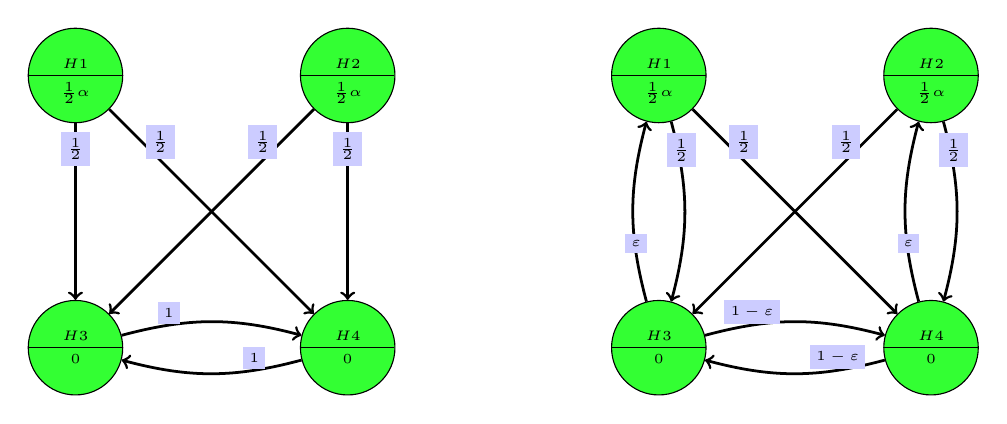
\begin{tikzpicture}[scale=0.7]
{\tiny

\node (H1) at (70bp,-70bp)[draw,circle split,minimum size=1.2cm, fill=green!80] {$H1$ \nodepart{lower} $\frac{1}{2}\alpha$};
\node (H2) at (210bp,-70bp)[draw,circle split,minimum size=1.2cm, fill=green!80] {$H2$ \nodepart{lower} $\frac{1}{2}\alpha$};
\node (H3) at (70bp,-210bp)[draw,circle split,minimum size=1.2cm, fill=green!80] {$H3$ \nodepart{lower} $0$};
\node (H4) at (210bp,-210bp)[draw,circle split,minimum size=1.2cm, fill=green!80] {$H4$ \nodepart{lower} $0$};
\draw [->,line width=1pt] (H1) to[auto] node[near start,above,fill=blue!20] {$\frac{1}{2}$} (H3);
\draw [->,line width=1pt] (H1) to[auto] node[near start,above,fill=blue!20] {$\frac{1}{2}$} (H4);
\draw [->,line width=1pt] (H2) to[auto] node[near start,above,fill=blue!20] {$\frac{1}{2}$} (H3);
\draw [->,line width=1pt] (H2) to[auto] node[near start,above,fill=blue!20] {$\frac{1}{2}$} (H4);
\draw [->,line width=1pt] (H3) to[bend left=15] node[near start,above,fill=blue!20] {$1$} (H4);
\draw [->,line width=1pt] (H4) to[bend left=15] node[near start,above,fill=blue!20] {$1$} (H3);
}{\tiny

\node (H1) at (370bp,-70bp)[draw,circle split,minimum size=1.2cm, fill=green!80] {$H1$ \nodepart{lower} $\frac{1}{2}\alpha$};
\node (H2) at (510bp,-70bp)[draw,circle split,minimum size=1.2cm, fill=green!80] {$H2$ \nodepart{lower} $\frac{1}{2}\alpha$};
\node (H3) at (370bp,-210bp)[draw,circle split,minimum size=1.2cm, fill=green!80] {$H3$ \nodepart{lower} $0$};
\node (H4) at (510bp,-210bp)[draw,circle split,minimum size=1.2cm, fill=green!80] {$H4$ \nodepart{lower} $0$};
\draw [->,line width=1pt] (H1) to[bend left=15] node[near start,above,fill=blue!20] {$\frac{1}{2}$} (H3);
\draw [->,line width=1pt] (H1) to[auto] node[near start,above,fill=blue!20] {$\frac{1}{2}$} (H4);
\draw [->,line width=1pt] (H2) to[auto] node[near start,above,fill=blue!20] {$\frac{1}{2}$} (H3);
\draw [->,line width=1pt] (H2) to[bend left=15] node[near start,above,fill=blue!20] {$\frac{1}{2}$} (H4);
\draw [->,line width=1pt] (H3) to[bend left=15] node[near start,above,fill=blue!20] {$1-\epsilon$} (H4);
\draw [->,line width=1pt] (H3) to[bend left=15] node[near start,above,fill=blue!20] {$\epsilon$} (H1);
\draw [->,line width=1pt] (H4) to[bend left=15] node[near start,above,fill=blue!20] {$1-\epsilon$} (H3);
\draw [->,line width=1pt] (H4) to[bend left=15] node[near start,above,fill=blue!20] {$\epsilon$} (H2);
}\end{tikzpicture}
  \caption{\label{gatekeeping}\index{parallel gatekeeping}\index{gatekeeping!parallel}\index{gatekeeping!improved parallel} The Parallel Gatekeeping and the Improved Parallel Gatekeeping Procedure.}
\end{figure}

\commentout{

Algorithm of Bretz et al. \cite{bretzEtAl2009power} for rejecting a node:

\[\alpha_l \leftarrow \begin{cases}\alpha_l+a_jg_{jl}&l\in I\\0&\text{otherwise}\end{cases}\]

\[g_{lk} \leftarrow \begin{cases}\frac{g_{lk}+g_{lj}g_{jk}}{1-g_{lj}g_{jl}}&k,l\in I, l\neq k, g_{lj}g_{jl}<1\\0&\text{otherwise}\end{cases}\]

We want now investigate what happens if a edge weight $\epsilon>0$ approaches $0$.
In respect to 

\[\alpha_l \leftarrow \begin{cases}0=\lim\limits_{g_{jl}\rightarrow0}(\alpha_l+a_jg_{jl})&l\in I\\0&\text{otherwise}\end{cases}\]

The only question is, what happens if and $l\in I, l\neq k, g_{lj}g_{jl}<1$.
If $g_{lj}g_{jl}==1$ still $g_{lk}<-0$.
 
\[\lim\limits_{g_{jl}\rightarrow0}\left(\frac{g_{lk}+g_{lj}g_{jk}}{1-g_{lj}g_{jl}}\right)
=\begin{cases}
  \frac{g_{lk}+g_{lj}g_{jk}}{1-g_{lj}g_{jl}}&g_{lj}g_{jl}<1\\
  0&g_{lj}g_{jl}=1\\a\\b\\\end{cases}
=\]
}


\scriptsize
\begin{Hchunk}
\begin{normalsize}
\begin{Hinput}
\ttfamily\noindent
\hlprompt{\usebox{\hlnormalsizeboxgreaterthan}{\ }}\hlsymbol{graph}{\ }\hlassignement{\usebox{\hlnormalsizeboxlessthan}-}{\ }\hlfunctioncall{createGraphForImprovedParallelGatekeeping}\hlkeyword{(}\hlkeyword{)}\mbox{}
\normalfont
\end{Hinput}


\begin{Hinput}
\ttfamily\noindent
\mbox{}
\normalfont
\end{Hinput}

\begin{Houtput}
\ttfamily\noindent
A{\ }graphMCP{\ }graph\hspace*{\fill}\\
\hlstd{}H1{\ }(not{\ }rejected,{\ }weight=0.5)\hspace*{\fill}\\
\hlstd{}H2{\ }(not{\ }rejected,{\ }weight=0.5)\hspace*{\fill}\\
\hlstd{}H3{\ }(not{\ }rejected,{\ }weight=0)\hspace*{\fill}\\
\hlstd{}H4{\ }(not{\ }rejected,{\ }weight=0)\hspace*{\fill}\\
\hlstd{}Edges:\hspace*{\fill}\\
\hlstd{}H1{\ }{\ }-({\ }1/2{\ })-\usebox{\hlnormalsizeboxgreaterthan}{\ }{\ }H3{\ }\hspace*{\fill}\\
\hlstd{}H1{\ }{\ }-({\ }1/2{\ })-\usebox{\hlnormalsizeboxgreaterthan}{\ }{\ }H4{\ }\hspace*{\fill}\\
\hlstd{}H2{\ }{\ }-({\ }1/2{\ })-\usebox{\hlnormalsizeboxgreaterthan}{\ }{\ }H3{\ }\hspace*{\fill}\\
\hlstd{}H2{\ }{\ }-({\ }1/2{\ })-\usebox{\hlnormalsizeboxgreaterthan}{\ }{\ }H4{\ }\hspace*{\fill}\\
\hlstd{}H3{\ }{\ }-({\ }1-\usebox{\hlnormalsizeboxbackslash}epsilon{\ })-\usebox{\hlnormalsizeboxgreaterthan}{\ }{\ }H4{\ }\hspace*{\fill}\\
\hlstd{}H3{\ }{\ }-({\ }\usebox{\hlnormalsizeboxbackslash}epsilon{\ })-\usebox{\hlnormalsizeboxgreaterthan}{\ }{\ }H1{\ }\hspace*{\fill}\\
\hlstd{}H4{\ }{\ }-({\ }1-\usebox{\hlnormalsizeboxbackslash}epsilon{\ })-\usebox{\hlnormalsizeboxgreaterthan}{\ }{\ }H3{\ }\hspace*{\fill}\\
\hlstd{}H4{\ }{\ }-({\ }\usebox{\hlnormalsizeboxbackslash}epsilon{\ })-\usebox{\hlnormalsizeboxgreaterthan}{\ }{\ }H2{\ }\hspace*{\fill}\hlstd{}\mbox{}
\normalfont
\end{Houtput}

\begin{Hinput}
\ttfamily\noindent
\hlprompt{\usebox{\hlnormalsizeboxgreaterthan}{\ }}\hlfunctioncall{substituteEps}\hlkeyword{(}\hlsymbol{graph}\hlkeyword{,}{\ }\hlargument{eps}\hlargument{=}\hlnumber{0.001}\hlkeyword{)}\mbox{}
\normalfont
\end{Hinput}

\begin{Houtput}
\ttfamily\noindent
A{\ }graphMCP{\ }graph\hspace*{\fill}\\
\hlstd{}H1{\ }(not{\ }rejected,{\ }weight=0.5)\hspace*{\fill}\\
\hlstd{}H2{\ }(not{\ }rejected,{\ }weight=0.5)\hspace*{\fill}\\
\hlstd{}H3{\ }(not{\ }rejected,{\ }weight=0)\hspace*{\fill}\\
\hlstd{}H4{\ }(not{\ }rejected,{\ }weight=0)\hspace*{\fill}\\
\hlstd{}Edges:\hspace*{\fill}\\
\hlstd{}H1{\ }{\ }-({\ }1/2{\ })-\usebox{\hlnormalsizeboxgreaterthan}{\ }{\ }H3{\ }\hspace*{\fill}\\
\hlstd{}H1{\ }{\ }-({\ }1/2{\ })-\usebox{\hlnormalsizeboxgreaterthan}{\ }{\ }H4{\ }\hspace*{\fill}\\
\hlstd{}H2{\ }{\ }-({\ }1/2{\ })-\usebox{\hlnormalsizeboxgreaterthan}{\ }{\ }H3{\ }\hspace*{\fill}\\
\hlstd{}H2{\ }{\ }-({\ }1/2{\ })-\usebox{\hlnormalsizeboxgreaterthan}{\ }{\ }H4{\ }\hspace*{\fill}\\
\hlstd{}H3{\ }{\ }-({\ }999/1000{\ })-\usebox{\hlnormalsizeboxgreaterthan}{\ }{\ }H4{\ }\hspace*{\fill}\\
\hlstd{}H3{\ }{\ }-({\ }1/1000{\ })-\usebox{\hlnormalsizeboxgreaterthan}{\ }{\ }H1{\ }\hspace*{\fill}\\
\hlstd{}H4{\ }{\ }-({\ }999/1000{\ })-\usebox{\hlnormalsizeboxgreaterthan}{\ }{\ }H3{\ }\hspace*{\fill}\\
\hlstd{}H4{\ }{\ }-({\ }1/1000{\ })-\usebox{\hlnormalsizeboxgreaterthan}{\ }{\ }H2{\ }\hspace*{\fill}\hlstd{}\mbox{}
\normalfont
\end{Houtput}

\begin{Hinput}
\ttfamily\noindent
\hlprompt{\usebox{\hlnormalsizeboxgreaterthan}{\ }}\hlfunctioncall{gMCP}\hlkeyword{(}\hlsymbol{graph}\hlkeyword{,}{\ }\hlargument{pvalues}\hlargument{=}\hlfunctioncall{c}\hlkeyword{(}\hlnumber{0.02}\hlkeyword{,}{\ }\hlnumber{0.04}\hlkeyword{,}{\ }\hlnumber{0.01}\hlkeyword{,}{\ }\hlnumber{0.02}\hlkeyword{)}\hlkeyword{,}{\ }\hlargument{eps}\hlargument{=}\hlnumber{0.001}\hlkeyword{)}\mbox{}
\normalfont
\end{Hinput}

\begin{Houtput}
\ttfamily\noindent
gMCP-Result\hspace*{\fill}\\
\hlstd{}\hspace*{\fill}\\
\hlstd{}Initial{\ }graph:\hspace*{\fill}\\
\hlstd{}A{\ }graphMCP{\ }graph\hspace*{\fill}\\
\hlstd{}H1{\ }(not{\ }rejected,{\ }weight=0.5)\hspace*{\fill}\\
\hlstd{}H2{\ }(not{\ }rejected,{\ }weight=0.5)\hspace*{\fill}\\
\hlstd{}H3{\ }(not{\ }rejected,{\ }weight=0)\hspace*{\fill}\\
\hlstd{}H4{\ }(not{\ }rejected,{\ }weight=0)\hspace*{\fill}\\
\hlstd{}Edges:\hspace*{\fill}\\
\hlstd{}H1{\ }{\ }-({\ }1/2{\ })-\usebox{\hlnormalsizeboxgreaterthan}{\ }{\ }H3{\ }\hspace*{\fill}\\
\hlstd{}H1{\ }{\ }-({\ }1/2{\ })-\usebox{\hlnormalsizeboxgreaterthan}{\ }{\ }H4{\ }\hspace*{\fill}\\
\hlstd{}H2{\ }{\ }-({\ }1/2{\ })-\usebox{\hlnormalsizeboxgreaterthan}{\ }{\ }H3{\ }\hspace*{\fill}\\
\hlstd{}H2{\ }{\ }-({\ }1/2{\ })-\usebox{\hlnormalsizeboxgreaterthan}{\ }{\ }H4{\ }\hspace*{\fill}\\
\hlstd{}H3{\ }{\ }-({\ }1-\usebox{\hlnormalsizeboxbackslash}epsilon{\ })-\usebox{\hlnormalsizeboxgreaterthan}{\ }{\ }H4{\ }\hspace*{\fill}\\
\hlstd{}H3{\ }{\ }-({\ }\usebox{\hlnormalsizeboxbackslash}epsilon{\ })-\usebox{\hlnormalsizeboxgreaterthan}{\ }{\ }H1{\ }\hspace*{\fill}\\
\hlstd{}H4{\ }{\ }-({\ }1-\usebox{\hlnormalsizeboxbackslash}epsilon{\ })-\usebox{\hlnormalsizeboxgreaterthan}{\ }{\ }H3{\ }\hspace*{\fill}\\
\hlstd{}H4{\ }{\ }-({\ }\usebox{\hlnormalsizeboxbackslash}epsilon{\ })-\usebox{\hlnormalsizeboxgreaterthan}{\ }{\ }H2{\ }\hspace*{\fill}\\
\hlstd{}\hspace*{\fill}\\
\hlstd{}\hspace*{\fill}\\
\hlstd{}P-values:\hspace*{\fill}\\
\hlstd{}{\ }{\ }H1{\ }{\ }{\ }H2{\ }{\ }{\ }H3{\ }{\ }{\ }H4{\ }\hspace*{\fill}\\
\hlstd{}0.02{\ }0.04{\ }0.01{\ }0.02{\ }\hspace*{\fill}\\
\hlstd{}\hspace*{\fill}\\
\hlstd{}Adjusted{\ }p-values:\hspace*{\fill}\\
\hlstd{}{\ }{\ }H1{\ }{\ }{\ }H2{\ }{\ }{\ }H3{\ }{\ }{\ }H4{\ }\hspace*{\fill}\\
\hlstd{}0.04{\ }0.04{\ }0.04{\ }0.04{\ }\hspace*{\fill}\\
\hlstd{}\hspace*{\fill}\\
\hlstd{}Alpha:{\ }0.05{\ }\hspace*{\fill}\\
\hlstd{}\hspace*{\fill}\\
\hlstd{}Hypothesis{\ }rejected:\hspace*{\fill}\\
\hlstd{}{\ }{\ }H1{\ }{\ }{\ }H2{\ }{\ }{\ }H3{\ }{\ }{\ }H4{\ }\hspace*{\fill}\\
\hlstd{}TRUE{\ }TRUE{\ }TRUE{\ }TRUE{\ }\hspace*{\fill}\\
\hlstd{}\hspace*{\fill}\\
\hlstd{}Final{\ }graph{\ }after{\ }4{\ }steps:\hspace*{\fill}\\
\hlstd{}A{\ }graphMCP{\ }graph\hspace*{\fill}\\
\hlstd{}H1{\ }(rejected,{\ }weight=0)\hspace*{\fill}\\
\hlstd{}H2{\ }(rejected,{\ }weight=1)\hspace*{\fill}\\
\hlstd{}H3{\ }(rejected,{\ }weight=0)\hspace*{\fill}\\
\hlstd{}H4{\ }(rejected,{\ }weight=0)\hspace*{\fill}\\
\hlstd{}No{\ }edges.\hspace*{\fill}\hlstd{}\mbox{}
\normalfont
\end{Houtput}

\end{normalsize}
\end{Hchunk}

\normalsize

\section{Power Simulations}\index{power simulation}

No $\epsilon$-edges are allowed.

\begin{figure}[ht]
  \centering   
{\tiny
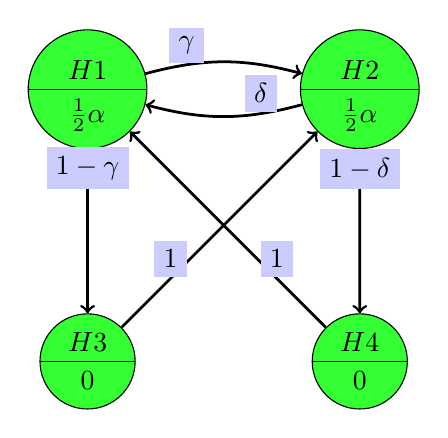
\begin{tikzpicture}[scale=0.7]
\node (H1) at (70bp,-70bp)[draw,circle split,fill=green!80] {$H1$ \nodepart{lower} $\frac{1}{2}\alpha$};
\node (H2) at (210bp,-70bp)[draw,circle split,fill=green!80] {$H2$ \nodepart{lower} $\frac{1}{2}\alpha$};
\node (H3) at (70bp,-210bp)[draw,circle split,fill=green!80] {$H3$ \nodepart{lower} $0$};
\node (H4) at (210bp,-210bp)[draw,circle split,fill=green!80] {$H4$ \nodepart{lower} $0$};
\draw [->,line width=1pt] (H1) to[bend left=15] node[near start,above,fill=blue!20] {$\gamma$} (H2);
\draw [->,line width=1pt] (H1) to[auto] node[near start,above,fill=blue!20] {$1-\gamma$} (H3);
\draw [->,line width=1pt] (H2) to[bend left=15] node[near start,above,fill=blue!20] {$\delta$} (H1);
\draw [->,line width=1pt] (H2) to[auto] node[near start,above,fill=blue!20] {$1-\delta$} (H4);
\draw [->,line width=1pt] (H3) to[auto] node[near start,above,fill=blue!20] {$1$} (H2);
\draw [->,line width=1pt] (H4) to[auto] node[near start,above,fill=blue!20] {$1$} (H1);
\end{tikzpicture}

}  \caption{\label{powergraph} Graph from Bretz et al. (2009)}
\end{figure}

\subsection{Variable edge weights}\index{edge weights!variable}

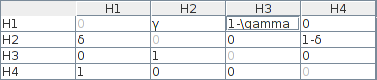
\includegraphics[width=0.5cm]{pictures/variableEditor.png}

\scriptsize
\begin{Hchunk}
\begin{normalsize}
\begin{Hinput}
\ttfamily\noindent
\hlprompt{\usebox{\hlnormalsizeboxgreaterthan}{\ }}\hlsymbol{graph}{\ }\hlassignement{\usebox{\hlnormalsizeboxlessthan}-}{\ }\hlfunctioncall{createGraph2FromBretzEtAl}\hlkeyword{(}\hlkeyword{)}\mbox{}
\normalfont
\end{Hinput}


\begin{Hinput}
\ttfamily\noindent
\mbox{}
\normalfont
\end{Hinput}

\begin{Houtput}
\ttfamily\noindent
A{\ }graphMCP{\ }graph\hspace*{\fill}\\
\hlstd{}H1{\ }(not{\ }rejected,{\ }weight=0.5)\hspace*{\fill}\\
\hlstd{}H2{\ }(not{\ }rejected,{\ }weight=0.5)\hspace*{\fill}\\
\hlstd{}H3{\ }(not{\ }rejected,{\ }weight=0)\hspace*{\fill}\\
\hlstd{}H4{\ }(not{\ }rejected,{\ }weight=0)\hspace*{\fill}\\
\hlstd{}Edges:\hspace*{\fill}\\
\hlstd{}H1{\ }{\ }-({\ }\usebox{\hlnormalsizeboxbackslash}gamma{\ })-\usebox{\hlnormalsizeboxgreaterthan}{\ }{\ }H2{\ }\hspace*{\fill}\\
\hlstd{}H1{\ }{\ }-({\ }1-\usebox{\hlnormalsizeboxbackslash}gamma{\ })-\usebox{\hlnormalsizeboxgreaterthan}{\ }{\ }H3{\ }\hspace*{\fill}\\
\hlstd{}H2{\ }{\ }-({\ }\usebox{\hlnormalsizeboxbackslash}delta{\ })-\usebox{\hlnormalsizeboxgreaterthan}{\ }{\ }H1{\ }\hspace*{\fill}\\
\hlstd{}H2{\ }{\ }-({\ }1-\usebox{\hlnormalsizeboxbackslash}delta{\ })-\usebox{\hlnormalsizeboxgreaterthan}{\ }{\ }H4{\ }\hspace*{\fill}\\
\hlstd{}H3{\ }{\ }-({\ }1{\ })-\usebox{\hlnormalsizeboxgreaterthan}{\ }{\ }H2{\ }\hspace*{\fill}\\
\hlstd{}H4{\ }{\ }-({\ }1{\ })-\usebox{\hlnormalsizeboxgreaterthan}{\ }{\ }H1{\ }\hspace*{\fill}\hlstd{}\mbox{}
\normalfont
\end{Houtput}

\end{normalsize}
\end{Hchunk}

\normalsize

\section{Options and Import/Export}

\subsection{Options}\index{options}

This subsection is work in progress, but fortunately the options in figure \ref{optionsDialog} should be fairly self-explanatory.

\begin{figure}[ht]
  \centering    
  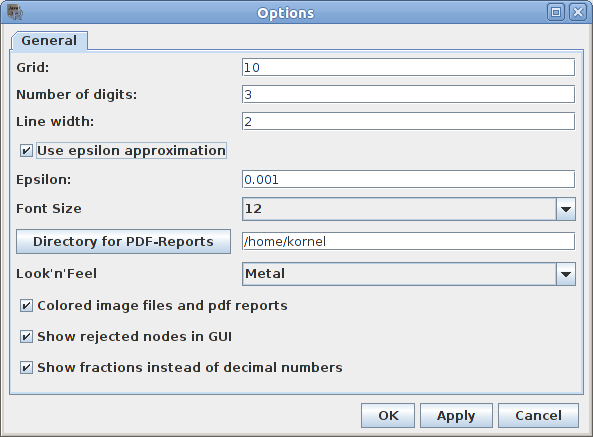
\includegraphics[width=0.7\textwidth]{pictures/optionsDialog.png}      
  \caption{\label{optionsDialog} You can configure many things in the option dialog.}
\end{figure}

\subsection{Import/Exports}\index{import}\index{export}

This subsection is work in progress, but fortunately the menu entries in figure \ref{fileMenu} should be fairly self-explanatory.

You can export graphs to png files.
The background of these png files will be made transperant, so that they will fit into whichever document you insert them.
Note that some image viewers visualize transparency with a checkerboard pattern.

\begin{figure}[ht]
  \centering    
  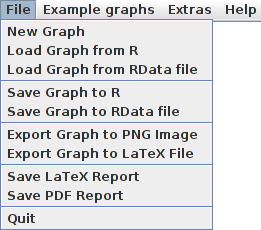
\includegraphics[width=4cm]{pictures/filemenu.png}      
  \caption{\label{fileMenu} Import and export of graphs.}
\end{figure}

\subsection{Important TikZ commands for optimizing the reports}\index{graph2latex}\index{TikZ}
A clear automatic placement of edges and weight labels without
overlapping is a very difficult task and for complicated graphs the
\texttt{gMCP} package will often fail to accomplish this.  There is
the possibilty to adjust the edges and labels in the GUI, but since
the {\LaTeX} graph layout is not (yet) exactly the same, there is
perhaps the need for adjusting the graphs in the TikZ code.  The TikZ
program is very useful and we recommend it for many purposes, but
perhaps you don't have the time to read the 560 pages manual
\cite{TikZ}, so here is a short overview of the most important
commands for this kind of graphs.

Let's start with this graph in figure \ref{uglygraph}:

\scriptsize
\lstset{language=[LaTeX]TeX}
\begin{lstlisting}
\begin{tikzpicture}[scale=1]
\node (H11) at (200bp,200bp) [draw,circle split,fill=green!80] {$H11$ \nodepart{lower} $0.0333$};
...
\draw [->,line width=1pt] (H11) to[bend left=15] node[near start,above,fill=blue!20] {0.667} (H12);
...
\end{tikzpicture}
\end{lstlisting}
\normalsize

\begin{figure}[ht]
  \centering   
{\tiny
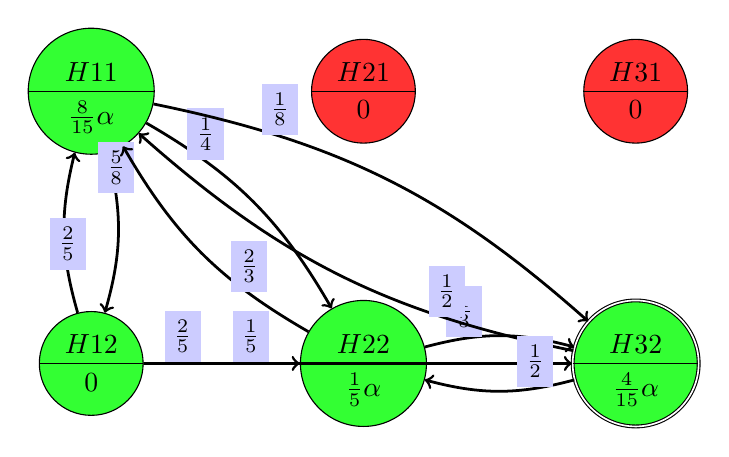
\begin{tikzpicture}[scale=0.7]
\node (H11) at (70bp,-70bp)[draw,circle split,fill=green!80] {$H11$ \nodepart{lower} $\frac{8}{15}\alpha$};
\node (H21) at (210bp,-70bp)[draw,circle split,fill=red!80] {$H21$ \nodepart{lower} $0$};
\node (H31) at (350bp,-70bp)[draw,circle split,fill=red!80] {$H31$ \nodepart{lower} $0$};
\node (H12) at (70bp,-210bp)[draw,circle split,fill=green!80] {$H12$ \nodepart{lower} $0$};
\node (H22) at (210bp,-210bp)[draw,circle split,fill=green!80] {$H22$ \nodepart{lower} $\frac{1}{5}\alpha$};
\node (H32) at (350bp,-210bp)[draw,circle split,double,fill=green!80] {$H32$ \nodepart{lower} $\frac{4}{15}\alpha$};
\draw [->,line width=1pt] (H11) to[bend left=15] node[near start,above,fill=blue!20] {$\frac{5}{8}$} (H12);
\draw [->,line width=1pt] (H11) to[bend left=15] node[near start,above,fill=blue!20] {$\frac{1}{4}$} (H22);
\draw [->,line width=1pt] (H11) to[bend left=15] node[near start,above,fill=blue!20] {$\frac{1}{8}$} (H32);
\draw [->,line width=1pt] (H12) to[bend left=15] node[near start,above,fill=blue!20] {$\frac{2}{5}$} (H11);
\draw [->,line width=1pt] (H12) to[auto] node[near start,above,fill=blue!20] {$\frac{2}{5}$} (H22);
\draw [->,line width=1pt] (H12) to[auto] node[near start,above,fill=blue!20] {$\frac{1}{5}$} (H32);
\draw [->,line width=1pt] (H22) to[bend left=15] node[near start,above,fill=blue!20] {$\frac{2}{3}$} (H11);
\draw [->,line width=1pt] (H22) to[bend left=15] node[near start,above,fill=blue!20] {$\frac{1}{3}$} (H32);
\draw [->,line width=1pt] (H32) to[bend left=15] node[near start,above,fill=blue!20] {$\frac{1}{2}$} (H11);
\draw [->,line width=1pt] (H32) to[bend left=15] node[near start,above,fill=blue!20] {$\frac{1}{2}$} (H22);
\end{tikzpicture}

}  \caption{\label{uglygraph}Graph from \texttt{graph2latex} that does not look optimal.}
\end{figure}

You can scale the TikZ graphic by changing the \texttt{[scale=1]}
option.  By default \texttt{graph2latex} doesn't scale TikZ graphics,
but has an optional parameter \texttt{scale}.

For an explanation what \texttt{green!80} means and how you can
specify other colors, please take a look at the xcolor manual
\cite{xcolor}.

You can choose between the following label positions \texttt{above,
  below, right, left, above right, above left, below right}, and
\texttt{below left}.  In addition these positions can take an optional
dimension argument, so that for example \texttt{below=1pt} can be used
to place a label below and additionally shift it 1pt downwards.

You can change the position where the edge weight label is placed to
\texttt{at start, very near start, near start, midway, near end, very
  near end} and \texttt{at end} or simply use something like
\texttt{pos=0.5}.  If you add an argument \texttt{sloped}, the text
label will be rotated so that a parallel line to the base line becomes
a tangent to the edge.

Often it is useful to reduce the bending angle in \texttt{[bend
    left=15]} below 15. You could also specify and change
\texttt{out=15} and \texttt{in=165} separately.

A powerful feature is the use of styles, since this will effect all
objects of a given class. But for this please take a look directly at
the TikZ manual \cite{TikZ}.

\section{Case Studies}\label{caseStudies}

This section is work in progress.

\begin{appendix} 

\section{Appendix - Multiple Testing Basics}

This section is work in progress.

\begin{Def}

\end{Def}

\end{appendix}

\newpage

\addcontentsline{toc}{section}{Index}
\printindex

\newpage

\addcontentsline{toc}{section}{Literatur}
\bibliography{literatur}

\end{document}
